% Options for packages loaded elsewhere
\PassOptionsToPackage{unicode}{hyperref}
\PassOptionsToPackage{hyphens}{url}
%
\documentclass[
]{article}
\usepackage{amsmath,amssymb}
\usepackage{lmodern}
\usepackage{iftex}
\ifPDFTeX
  \usepackage[T1]{fontenc}
  \usepackage[utf8]{inputenc}
  \usepackage{textcomp} % provide euro and other symbols
\else % if luatex or xetex
  \usepackage{unicode-math}
  \defaultfontfeatures{Scale=MatchLowercase}
  \defaultfontfeatures[\rmfamily]{Ligatures=TeX,Scale=1}
\fi
% Use upquote if available, for straight quotes in verbatim environments
\IfFileExists{upquote.sty}{\usepackage{upquote}}{}
\IfFileExists{microtype.sty}{% use microtype if available
  \usepackage[]{microtype}
  \UseMicrotypeSet[protrusion]{basicmath} % disable protrusion for tt fonts
}{}
\makeatletter
\@ifundefined{KOMAClassName}{% if non-KOMA class
  \IfFileExists{parskip.sty}{%
    \usepackage{parskip}
  }{% else
    \setlength{\parindent}{0pt}
    \setlength{\parskip}{6pt plus 2pt minus 1pt}}
}{% if KOMA class
  \KOMAoptions{parskip=half}}
\makeatother
\usepackage{xcolor}
\usepackage[margin=1in]{geometry}
\usepackage{color}
\usepackage{fancyvrb}
\newcommand{\VerbBar}{|}
\newcommand{\VERB}{\Verb[commandchars=\\\{\}]}
\DefineVerbatimEnvironment{Highlighting}{Verbatim}{commandchars=\\\{\}}
% Add ',fontsize=\small' for more characters per line
\usepackage{framed}
\definecolor{shadecolor}{RGB}{248,248,248}
\newenvironment{Shaded}{\begin{snugshade}}{\end{snugshade}}
\newcommand{\AlertTok}[1]{\textcolor[rgb]{0.94,0.16,0.16}{#1}}
\newcommand{\AnnotationTok}[1]{\textcolor[rgb]{0.56,0.35,0.01}{\textbf{\textit{#1}}}}
\newcommand{\AttributeTok}[1]{\textcolor[rgb]{0.77,0.63,0.00}{#1}}
\newcommand{\BaseNTok}[1]{\textcolor[rgb]{0.00,0.00,0.81}{#1}}
\newcommand{\BuiltInTok}[1]{#1}
\newcommand{\CharTok}[1]{\textcolor[rgb]{0.31,0.60,0.02}{#1}}
\newcommand{\CommentTok}[1]{\textcolor[rgb]{0.56,0.35,0.01}{\textit{#1}}}
\newcommand{\CommentVarTok}[1]{\textcolor[rgb]{0.56,0.35,0.01}{\textbf{\textit{#1}}}}
\newcommand{\ConstantTok}[1]{\textcolor[rgb]{0.00,0.00,0.00}{#1}}
\newcommand{\ControlFlowTok}[1]{\textcolor[rgb]{0.13,0.29,0.53}{\textbf{#1}}}
\newcommand{\DataTypeTok}[1]{\textcolor[rgb]{0.13,0.29,0.53}{#1}}
\newcommand{\DecValTok}[1]{\textcolor[rgb]{0.00,0.00,0.81}{#1}}
\newcommand{\DocumentationTok}[1]{\textcolor[rgb]{0.56,0.35,0.01}{\textbf{\textit{#1}}}}
\newcommand{\ErrorTok}[1]{\textcolor[rgb]{0.64,0.00,0.00}{\textbf{#1}}}
\newcommand{\ExtensionTok}[1]{#1}
\newcommand{\FloatTok}[1]{\textcolor[rgb]{0.00,0.00,0.81}{#1}}
\newcommand{\FunctionTok}[1]{\textcolor[rgb]{0.00,0.00,0.00}{#1}}
\newcommand{\ImportTok}[1]{#1}
\newcommand{\InformationTok}[1]{\textcolor[rgb]{0.56,0.35,0.01}{\textbf{\textit{#1}}}}
\newcommand{\KeywordTok}[1]{\textcolor[rgb]{0.13,0.29,0.53}{\textbf{#1}}}
\newcommand{\NormalTok}[1]{#1}
\newcommand{\OperatorTok}[1]{\textcolor[rgb]{0.81,0.36,0.00}{\textbf{#1}}}
\newcommand{\OtherTok}[1]{\textcolor[rgb]{0.56,0.35,0.01}{#1}}
\newcommand{\PreprocessorTok}[1]{\textcolor[rgb]{0.56,0.35,0.01}{\textit{#1}}}
\newcommand{\RegionMarkerTok}[1]{#1}
\newcommand{\SpecialCharTok}[1]{\textcolor[rgb]{0.00,0.00,0.00}{#1}}
\newcommand{\SpecialStringTok}[1]{\textcolor[rgb]{0.31,0.60,0.02}{#1}}
\newcommand{\StringTok}[1]{\textcolor[rgb]{0.31,0.60,0.02}{#1}}
\newcommand{\VariableTok}[1]{\textcolor[rgb]{0.00,0.00,0.00}{#1}}
\newcommand{\VerbatimStringTok}[1]{\textcolor[rgb]{0.31,0.60,0.02}{#1}}
\newcommand{\WarningTok}[1]{\textcolor[rgb]{0.56,0.35,0.01}{\textbf{\textit{#1}}}}
\usepackage{graphicx}
\makeatletter
\def\maxwidth{\ifdim\Gin@nat@width>\linewidth\linewidth\else\Gin@nat@width\fi}
\def\maxheight{\ifdim\Gin@nat@height>\textheight\textheight\else\Gin@nat@height\fi}
\makeatother
% Scale images if necessary, so that they will not overflow the page
% margins by default, and it is still possible to overwrite the defaults
% using explicit options in \includegraphics[width, height, ...]{}
\setkeys{Gin}{width=\maxwidth,height=\maxheight,keepaspectratio}
% Set default figure placement to htbp
\makeatletter
\def\fps@figure{htbp}
\makeatother
\setlength{\emergencystretch}{3em} % prevent overfull lines
\providecommand{\tightlist}{%
  \setlength{\itemsep}{0pt}\setlength{\parskip}{0pt}}
\setcounter{secnumdepth}{-\maxdimen} % remove section numbering
\usepackage{booktabs}
\usepackage{longtable}
\usepackage{array}
\usepackage{multirow}
\usepackage{wrapfig}
\usepackage{float}
\usepackage{colortbl}
\usepackage{pdflscape}
\usepackage{tabu}
\usepackage{threeparttable}
\usepackage{threeparttablex}
\usepackage[normalem]{ulem}
\usepackage{makecell}
\usepackage{xcolor}
\usepackage{siunitx}

  \newcolumntype{d}{S[
    input-open-uncertainty=,
    input-close-uncertainty=,
    parse-numbers = false,
    table-align-text-pre=false,
    table-align-text-post=false
  ]}
  
\ifLuaTeX
  \usepackage{selnolig}  % disable illegal ligatures
\fi
\IfFileExists{bookmark.sty}{\usepackage{bookmark}}{\usepackage{hyperref}}
\IfFileExists{xurl.sty}{\usepackage{xurl}}{} % add URL line breaks if available
\urlstyle{same} % disable monospaced font for URLs
\hypersetup{
  pdftitle={Predicting Student Dropouts},
  pdfauthor={Mahathi Gandhamaneni},
  hidelinks,
  pdfcreator={LaTeX via pandoc}}

\title{Predicting Student Dropouts}
\author{Mahathi Gandhamaneni}
\date{March 13th, 2023}

\begin{document}
\maketitle

\hypertarget{introduction}{%
\section{Introduction}\label{introduction}}

In recent times, there has been a spotlight on the inequity that
students face during university - whether that be during the admissions
process, or throughout the rest of their studies once they are in.

In particular, the opportunities that seem to be available to everyone
regardless of who they are or where they are from, may just be a mirage.
Through taking a look at the news and articles, it appears that not just
academics, but demographic, socioeconomic, and macroeconomic factors
appear to have an effect on students in university. For example,
students coming from certain backgrounds may not have financial,
academic, or even emotional support being provided by their families.

Sometimes, these factors may lead to a student dropping out or they may
lead to a student graduating with honours. What we want to investigate
here is whether we can predict what outcome a student will face based on
certain socioeconomic, demographic, and macroeconomic factors.
Specifically, the question we want to answer in this project is as
follows: \textbf{Can we predict whether a student will drop out of an
undergraduate degree program or not, based on factors such as gender,
unemployment rates, nationality, 2019 life expectancy (based on
nationality), previous qualification, mother's and father's
qualification, and program of study?}

\hypertarget{methods}{%
\section{Methods}\label{methods}}

\hypertarget{data-collection}{%
\subsection{Data Collection}\label{data-collection}}

The data was primarily acquired from two sources: a Kaggle dataset
entitled ``Predict students' dropout and academic success''
(\url{https://www.kaggle.com/datasets/thedevastator/higher-education-predictors-of-student-retention?datasetId=2780494\&searchQuery=cleaning})
which I will henceforth refer to as the ``Student Data'', and 2019 life
expectancy data extracted using the World Bank Gender Data Portal API
(which I will refer to as the ``World Bank Data'').

The main data is actually derived from a dataset created by Realinho et
al (2022) for their paper entitled Predicting Student Dropout and
Academic Success (Realinho et al). This paper is where I was able to
find all the background information about the dataset for the purposes
of understanding it, and using it to perform data analysis. The dataset
was developed at the Polytechnic Institute of Portalegre and was used to
build machine learning models to predict academic performance. The data
in the dataset was derived from several sources of academic (student),
socioeconomic, and macroeconomic data in Portugal (Realinho et al can be
consulted for more detail into the sources). It refers to student
records enrolled between the academic years of 2008 to 2019. Almost all
the categorical variables in the dataset are numerically encoded (the
numeric encoding values are found at
\url{https://www.mdpi.com/2306-5729/7/11/146}). In order to simplify
data exploration and analysis, as well as enhance readability, we have
decided to replace the numeric encoding with the real values. The main
data does not have a reference to the year from which an observation was
extracted, so it is very difficult to figure out what year of life
expectancy data to associate with which record. In order to simplify the
process (even though it may be at the expense of accuracy), 2019 life
expectancy figures were used for every observation respective to their
nationality.

Within the World Bank API, every country is assigned a three letter ISO
code which allows us to concatenate the appropriate URL for each country
so that we can extract the life expectancy data for 2019. For any given
country, the API link for the average life expectancy in 2019 is as
follows: ``\url{http://api.worldbank.org/v2/country/\%5BISO} COUNTRY
CODE{]}/indicator/SP.DYN.LE00.IN?date=2019'', where {[}ISO COUNTRY
CODE{]} is a standardized code system followed worldwide. The main data
exhibits that the student demographic within the data was no more than
21 nationalities. Looking at these 21 values, we can find the ISO code
for each one of the countries, and iterate through them all, extracting
the appropriate figures and storing them in a dataframe. After this
process of data extraction, the main data and the world bank data were
then merged through a left join on the nationalities, so that each
observation in the final dataframe had a 2019 life expectancy value
associated with it based on the student's nationality.

\hypertarget{data-cleaning-wrangling}{%
\subsection{Data Cleaning \& Wrangling}\label{data-cleaning-wrangling}}

Since the main data was already used in analysis and modelling in a
prior study, it was already cleaned and prepared well. There were no
missing values or any other immediate issues that needed to be addressed
before the data could be used. However, there were quite a few columns
in the main data that we will not be using in our analysis that needed
to be dropped from the data frame.

In fact, of the 35 variables in the main dataset, the only variables
selected were:

\begin{enumerate}
\item Course: The course taken by the student. (Categorical)
\item Previous qualification: The qualification obtained by the student before enrolling in higher education. (Categorical)
\item Nationality: The nationality of the student. (Categorical)
\item Mother's qualification: The qualification of the student's mother. (Categorical)
\item Father's qualification: The qualification of the student's father. (Categorical)
\item Gender: The gender of the student. (Categorical)
\item Age at enrollment: The age of the student at the time of enrollment. (Numerical)
\item Unemployment rate: Unemployment rate at the time the data was recorded. (Numerical)
\item Target: The status of the student (enrolled, dropped out, or graduated) (Categorical)
\end{enumerate}

Some of the variables within the main data were also renamed to minimize
length and to also increase readability.

Similarly, when it comes to the life expectancy data frame that we
extracted, there were columns that were unnecessary and that needed to
be dropped. Specifically, we were interested in only two columns - the
ISO country code (which served as a unique identifier until an ID column
was added) and the actual life expectancy value column. An ID column was
added to this dataframe in order to match the nationality encoding in
the main dataset to make merging the two easier. After the two
dataframes were merged, the ISO country code column was removed, thus
leaving only the life expectancy value that we need.

\hypertarget{data-exploration}{%
\subsection{Data Exploration}\label{data-exploration}}

Now that we have our cleaned and wrangled data, we can begin to explore
key variables and associations.

In total, the dataset has 4424 observations and 10 variables. In order
to explore the data, we decided to take a look at the distributions of
all the variables, frequencies of categorical variables, and summary
statistics for numerical variables. Specifically, we explored the
variables Course, Previous qualification, Mother's qualification, and
Father's qualification through bar plots and frequency tables. We
explored the numerical variables Age, Unemployment rate, and Life
expectancy through histograms and summary statistics tables. As for the
variables gender and target, we used frequency tables to examine these
since they have comparatively fewer categories as compared to the other
variables in the data set and their composition can be understood
through looking at the frequency of their values.

\hypertarget{preliminary-results}{%
\section{Preliminary Results}\label{preliminary-results}}

\begin{Shaded}
\begin{Highlighting}[]
\CommentTok{\# undoing numerical encoding}

\CommentTok{\# nationality}
\NormalTok{df}\SpecialCharTok{$}\NormalTok{Nationality[df}\SpecialCharTok{$}\NormalTok{Nationality }\SpecialCharTok{==} \StringTok{"1"}\NormalTok{] }\OtherTok{\textless{}{-}} \StringTok{"Portuguese"}
\NormalTok{df}\SpecialCharTok{$}\NormalTok{Nationality[df}\SpecialCharTok{$}\NormalTok{Nationality }\SpecialCharTok{==} \StringTok{"2"}\NormalTok{] }\OtherTok{\textless{}{-}} \StringTok{"German"}
\NormalTok{df}\SpecialCharTok{$}\NormalTok{Nationality[df}\SpecialCharTok{$}\NormalTok{Nationality }\SpecialCharTok{==} \StringTok{"3"}\NormalTok{] }\OtherTok{\textless{}{-}} \StringTok{"Spanish"}
\NormalTok{df}\SpecialCharTok{$}\NormalTok{Nationality[df}\SpecialCharTok{$}\NormalTok{Nationality }\SpecialCharTok{==} \StringTok{"4"}\NormalTok{] }\OtherTok{\textless{}{-}} \StringTok{"Italian"}
\NormalTok{df}\SpecialCharTok{$}\NormalTok{Nationality[df}\SpecialCharTok{$}\NormalTok{Nationality }\SpecialCharTok{==} \StringTok{"5"}\NormalTok{] }\OtherTok{\textless{}{-}} \StringTok{"Dutch"}
\NormalTok{df}\SpecialCharTok{$}\NormalTok{Nationality[df}\SpecialCharTok{$}\NormalTok{Nationality }\SpecialCharTok{==} \StringTok{"6"}\NormalTok{] }\OtherTok{\textless{}{-}} \StringTok{"English"}
\NormalTok{df}\SpecialCharTok{$}\NormalTok{Nationality[df}\SpecialCharTok{$}\NormalTok{Nationality }\SpecialCharTok{==} \StringTok{"7"}\NormalTok{] }\OtherTok{\textless{}{-}} \StringTok{"Lithuanian"}
\NormalTok{df}\SpecialCharTok{$}\NormalTok{Nationality[df}\SpecialCharTok{$}\NormalTok{Nationality }\SpecialCharTok{==} \StringTok{"8"}\NormalTok{] }\OtherTok{\textless{}{-}} \StringTok{"Angolan"}
\NormalTok{df}\SpecialCharTok{$}\NormalTok{Nationality[df}\SpecialCharTok{$}\NormalTok{Nationality }\SpecialCharTok{==} \StringTok{"9"}\NormalTok{] }\OtherTok{\textless{}{-}} \StringTok{"Cape Verdean"}
\NormalTok{df}\SpecialCharTok{$}\NormalTok{Nationality[df}\SpecialCharTok{$}\NormalTok{Nationality }\SpecialCharTok{==} \StringTok{"10"}\NormalTok{] }\OtherTok{\textless{}{-}} \StringTok{"Guinean"}
\NormalTok{df}\SpecialCharTok{$}\NormalTok{Nationality[df}\SpecialCharTok{$}\NormalTok{Nationality }\SpecialCharTok{==} \StringTok{"11"}\NormalTok{] }\OtherTok{\textless{}{-}} \StringTok{"Mozambican"}
\NormalTok{df}\SpecialCharTok{$}\NormalTok{Nationality[df}\SpecialCharTok{$}\NormalTok{Nationality }\SpecialCharTok{==} \StringTok{"12"}\NormalTok{] }\OtherTok{\textless{}{-}} \StringTok{"Santomean"}
\NormalTok{df}\SpecialCharTok{$}\NormalTok{Nationality[df}\SpecialCharTok{$}\NormalTok{Nationality }\SpecialCharTok{==} \StringTok{"13"}\NormalTok{] }\OtherTok{\textless{}{-}} \StringTok{"Turkish"}
\NormalTok{df}\SpecialCharTok{$}\NormalTok{Nationality[df}\SpecialCharTok{$}\NormalTok{Nationality }\SpecialCharTok{==} \StringTok{"14"}\NormalTok{] }\OtherTok{\textless{}{-}} \StringTok{"Brazilian"}
\NormalTok{df}\SpecialCharTok{$}\NormalTok{Nationality[df}\SpecialCharTok{$}\NormalTok{Nationality }\SpecialCharTok{==} \StringTok{"15"}\NormalTok{] }\OtherTok{\textless{}{-}} \StringTok{"Romanian"}
\NormalTok{df}\SpecialCharTok{$}\NormalTok{Nationality[df}\SpecialCharTok{$}\NormalTok{Nationality }\SpecialCharTok{==} \StringTok{"16"}\NormalTok{] }\OtherTok{\textless{}{-}} \StringTok{"Moldova (Republic of)"}
\NormalTok{df}\SpecialCharTok{$}\NormalTok{Nationality[df}\SpecialCharTok{$}\NormalTok{Nationality }\SpecialCharTok{==} \StringTok{"17"}\NormalTok{] }\OtherTok{\textless{}{-}} \StringTok{"Mexican"}
\NormalTok{df}\SpecialCharTok{$}\NormalTok{Nationality[df}\SpecialCharTok{$}\NormalTok{Nationality }\SpecialCharTok{==} \StringTok{"18"}\NormalTok{] }\OtherTok{\textless{}{-}} \StringTok{"Ukrainian"}
\NormalTok{df}\SpecialCharTok{$}\NormalTok{Nationality[df}\SpecialCharTok{$}\NormalTok{Nationality }\SpecialCharTok{==} \StringTok{"19"}\NormalTok{] }\OtherTok{\textless{}{-}} \StringTok{"Russian"}
\NormalTok{df}\SpecialCharTok{$}\NormalTok{Nationality[df}\SpecialCharTok{$}\NormalTok{Nationality }\SpecialCharTok{==} \StringTok{"20"}\NormalTok{] }\OtherTok{\textless{}{-}} \StringTok{"Cuban"}
\NormalTok{df}\SpecialCharTok{$}\NormalTok{Nationality[df}\SpecialCharTok{$}\NormalTok{Nationality }\SpecialCharTok{==} \StringTok{"21"}\NormalTok{] }\OtherTok{\textless{}{-}} \StringTok{"Colombian"}

\CommentTok{\#course}
\NormalTok{df}\SpecialCharTok{$}\NormalTok{Program[df}\SpecialCharTok{$}\NormalTok{Program }\SpecialCharTok{==} \StringTok{"1"}\NormalTok{] }\OtherTok{\textless{}{-}} \StringTok{"Biofuel Production Technologies"}
\NormalTok{df}\SpecialCharTok{$}\NormalTok{Program[df}\SpecialCharTok{$}\NormalTok{Program }\SpecialCharTok{==} \StringTok{"2"}\NormalTok{] }\OtherTok{\textless{}{-}} \StringTok{"Animation and Multimedia Design"}
\NormalTok{df}\SpecialCharTok{$}\NormalTok{Program[df}\SpecialCharTok{$}\NormalTok{Program }\SpecialCharTok{==} \StringTok{"3"}\NormalTok{] }\OtherTok{\textless{}{-}} \StringTok{"Social Service (evening attendance)"}
\NormalTok{df}\SpecialCharTok{$}\NormalTok{Program[df}\SpecialCharTok{$}\NormalTok{Program }\SpecialCharTok{==} \StringTok{"4"}\NormalTok{] }\OtherTok{\textless{}{-}} \StringTok{"Agronomy"}
\NormalTok{df}\SpecialCharTok{$}\NormalTok{Program[df}\SpecialCharTok{$}\NormalTok{Program }\SpecialCharTok{==} \StringTok{"5"}\NormalTok{] }\OtherTok{\textless{}{-}} \StringTok{"Communication Design"}
\NormalTok{df}\SpecialCharTok{$}\NormalTok{Program[df}\SpecialCharTok{$}\NormalTok{Program }\SpecialCharTok{==} \StringTok{"6"}\NormalTok{] }\OtherTok{\textless{}{-}} \StringTok{"Veterinary Nursing"}
\NormalTok{df}\SpecialCharTok{$}\NormalTok{Program[df}\SpecialCharTok{$}\NormalTok{Program }\SpecialCharTok{==} \StringTok{"7"}\NormalTok{] }\OtherTok{\textless{}{-}} \StringTok{"Informatics Engineering"}
\NormalTok{df}\SpecialCharTok{$}\NormalTok{Program[df}\SpecialCharTok{$}\NormalTok{Program }\SpecialCharTok{==} \StringTok{"8"}\NormalTok{] }\OtherTok{\textless{}{-}} \StringTok{"Equiniculture"}
\NormalTok{df}\SpecialCharTok{$}\NormalTok{Program[df}\SpecialCharTok{$}\NormalTok{Program }\SpecialCharTok{==} \StringTok{"9"}\NormalTok{] }\OtherTok{\textless{}{-}} \StringTok{"Management"}
\NormalTok{df}\SpecialCharTok{$}\NormalTok{Program[df}\SpecialCharTok{$}\NormalTok{Program }\SpecialCharTok{==} \StringTok{"10"}\NormalTok{] }\OtherTok{\textless{}{-}} \StringTok{"Social Service"}
\NormalTok{df}\SpecialCharTok{$}\NormalTok{Program[df}\SpecialCharTok{$}\NormalTok{Program }\SpecialCharTok{==} \StringTok{"11"}\NormalTok{] }\OtherTok{\textless{}{-}} \StringTok{"Tourism"}
\NormalTok{df}\SpecialCharTok{$}\NormalTok{Program[df}\SpecialCharTok{$}\NormalTok{Program }\SpecialCharTok{==} \StringTok{"12"}\NormalTok{] }\OtherTok{\textless{}{-}} \StringTok{"Nursing"}
\NormalTok{df}\SpecialCharTok{$}\NormalTok{Program[df}\SpecialCharTok{$}\NormalTok{Program }\SpecialCharTok{==} \StringTok{"13"}\NormalTok{] }\OtherTok{\textless{}{-}} \StringTok{"Oral Hygiene"}
\NormalTok{df}\SpecialCharTok{$}\NormalTok{Program[df}\SpecialCharTok{$}\NormalTok{Program }\SpecialCharTok{==} \StringTok{"14"}\NormalTok{] }\OtherTok{\textless{}{-}} \StringTok{"Advertising and Marketing Management"}
\NormalTok{df}\SpecialCharTok{$}\NormalTok{Program[df}\SpecialCharTok{$}\NormalTok{Program }\SpecialCharTok{==} \StringTok{"15"}\NormalTok{] }\OtherTok{\textless{}{-}} \StringTok{"Journalism and Communication"}
\NormalTok{df}\SpecialCharTok{$}\NormalTok{Program[df}\SpecialCharTok{$}\NormalTok{Program }\SpecialCharTok{==} \StringTok{"16"}\NormalTok{] }\OtherTok{\textless{}{-}} \StringTok{"Basic Education"}
\NormalTok{df}\SpecialCharTok{$}\NormalTok{Program[df}\SpecialCharTok{$}\NormalTok{Program }\SpecialCharTok{==} \StringTok{"17"}\NormalTok{] }\OtherTok{\textless{}{-}} \StringTok{"Management (evening attendance)"}

\CommentTok{\#prev quali}
\NormalTok{df}\SpecialCharTok{$}\NormalTok{Prev\_quali[df}\SpecialCharTok{$}\NormalTok{Prev\_quali }\SpecialCharTok{==} \StringTok{"1"}\NormalTok{] }\OtherTok{\textless{}{-}} \StringTok{"Secondary education"}
\NormalTok{df}\SpecialCharTok{$}\NormalTok{Prev\_quali[df}\SpecialCharTok{$}\NormalTok{Prev\_quali }\SpecialCharTok{==} \StringTok{"2"}\NormalTok{] }\OtherTok{\textless{}{-}} \StringTok{"Higher education—bachelor’s degree"}
\NormalTok{df}\SpecialCharTok{$}\NormalTok{Prev\_quali[df}\SpecialCharTok{$}\NormalTok{Prev\_quali }\SpecialCharTok{==} \StringTok{"3"}\NormalTok{] }\OtherTok{\textless{}{-}} \StringTok{"Higher education—degree"}
\NormalTok{df}\SpecialCharTok{$}\NormalTok{Prev\_quali[df}\SpecialCharTok{$}\NormalTok{Prev\_quali }\SpecialCharTok{==} \StringTok{"4"}\NormalTok{] }\OtherTok{\textless{}{-}} \StringTok{"Higher education—master’s degree"}
\NormalTok{df}\SpecialCharTok{$}\NormalTok{Prev\_quali[df}\SpecialCharTok{$}\NormalTok{Prev\_quali }\SpecialCharTok{==} \StringTok{"5"}\NormalTok{] }\OtherTok{\textless{}{-}} \StringTok{"Higher education—doctorate"}
\NormalTok{df}\SpecialCharTok{$}\NormalTok{Prev\_quali[df}\SpecialCharTok{$}\NormalTok{Prev\_quali }\SpecialCharTok{==} \StringTok{"6"}\NormalTok{] }\OtherTok{\textless{}{-}} \StringTok{"Frequency of higher education"}
\NormalTok{df}\SpecialCharTok{$}\NormalTok{Prev\_quali[df}\SpecialCharTok{$}\NormalTok{Prev\_quali }\SpecialCharTok{==} \StringTok{"7"}\NormalTok{] }\OtherTok{\textless{}{-}} \StringTok{"12th year of schooling—not completed"}
\NormalTok{df}\SpecialCharTok{$}\NormalTok{Prev\_quali[df}\SpecialCharTok{$}\NormalTok{Prev\_quali }\SpecialCharTok{==} \StringTok{"8"}\NormalTok{] }\OtherTok{\textless{}{-}} \StringTok{"11th year of schooling—not completed"}
\NormalTok{df}\SpecialCharTok{$}\NormalTok{Prev\_quali[df}\SpecialCharTok{$}\NormalTok{Prev\_quali }\SpecialCharTok{==} \StringTok{"9"}\NormalTok{] }\OtherTok{\textless{}{-}} \StringTok{"Other—11th year of schooling"}
\NormalTok{df}\SpecialCharTok{$}\NormalTok{Prev\_quali[df}\SpecialCharTok{$}\NormalTok{Prev\_quali }\SpecialCharTok{==} \StringTok{"10"}\NormalTok{] }\OtherTok{\textless{}{-}} \StringTok{"10th year of schooling"}
\NormalTok{df}\SpecialCharTok{$}\NormalTok{Prev\_quali[df}\SpecialCharTok{$}\NormalTok{Prev\_quali }\SpecialCharTok{==} \StringTok{"11"}\NormalTok{] }\OtherTok{\textless{}{-}} \StringTok{"10th year of schooling—not completed"}
\NormalTok{df}\SpecialCharTok{$}\NormalTok{Prev\_quali[df}\SpecialCharTok{$}\NormalTok{Prev\_quali }\SpecialCharTok{==} \StringTok{"12"}\NormalTok{] }\OtherTok{\textless{}{-}} \StringTok{"Basic education 3rd cycle (9th/10th/11th year) or equivalent"}
\NormalTok{df}\SpecialCharTok{$}\NormalTok{Prev\_quali[df}\SpecialCharTok{$}\NormalTok{Prev\_quali }\SpecialCharTok{==} \StringTok{"13"}\NormalTok{] }\OtherTok{\textless{}{-}} \StringTok{"Basic education 2nd cycle (6th/7th/8th year) or equivalent"}
\NormalTok{df}\SpecialCharTok{$}\NormalTok{Prev\_quali[df}\SpecialCharTok{$}\NormalTok{Prev\_quali }\SpecialCharTok{==} \StringTok{"14"}\NormalTok{] }\OtherTok{\textless{}{-}} \StringTok{"Technological specialization course"}
\NormalTok{df}\SpecialCharTok{$}\NormalTok{Prev\_quali[df}\SpecialCharTok{$}\NormalTok{Prev\_quali }\SpecialCharTok{==} \StringTok{"15"}\NormalTok{] }\OtherTok{\textless{}{-}} \StringTok{"Higher education—degree (1st cycle)"}
\NormalTok{df}\SpecialCharTok{$}\NormalTok{Prev\_quali[df}\SpecialCharTok{$}\NormalTok{Prev\_quali }\SpecialCharTok{==} \StringTok{"16"}\NormalTok{] }\OtherTok{\textless{}{-}} \StringTok{"Professional higher technical course"}
\NormalTok{df}\SpecialCharTok{$}\NormalTok{Prev\_quali[df}\SpecialCharTok{$}\NormalTok{Prev\_quali }\SpecialCharTok{==} \StringTok{"17"}\NormalTok{] }\OtherTok{\textless{}{-}} \StringTok{"Higher education—master’s degree (2nd cycle)"}

\CommentTok{\#mothers quali}
\NormalTok{df}\SpecialCharTok{$}\NormalTok{Mom\_quali[df}\SpecialCharTok{$}\NormalTok{Mom\_quali }\SpecialCharTok{==} \StringTok{"1"}\NormalTok{] }\OtherTok{\textless{}{-}} \StringTok{"Secondary Education—12th Year of Schooling or Equivalent"}
\NormalTok{df}\SpecialCharTok{$}\NormalTok{Mom\_quali[df}\SpecialCharTok{$}\NormalTok{Mom\_quali }\SpecialCharTok{==} \StringTok{"2"}\NormalTok{] }\OtherTok{\textless{}{-}} \StringTok{"Higher Education—bachelor’s degree"}
\NormalTok{df}\SpecialCharTok{$}\NormalTok{Mom\_quali[df}\SpecialCharTok{$}\NormalTok{Mom\_quali }\SpecialCharTok{==} \StringTok{"3"}\NormalTok{] }\OtherTok{\textless{}{-}} \StringTok{"Higher Education—degree"}
\NormalTok{df}\SpecialCharTok{$}\NormalTok{Mom\_quali[df}\SpecialCharTok{$}\NormalTok{Mom\_quali }\SpecialCharTok{==} \StringTok{"4"}\NormalTok{] }\OtherTok{\textless{}{-}} \StringTok{"Higher Education—master’s degree"}
\NormalTok{df}\SpecialCharTok{$}\NormalTok{Mom\_quali[df}\SpecialCharTok{$}\NormalTok{Mom\_quali }\SpecialCharTok{==} \StringTok{"5"}\NormalTok{] }\OtherTok{\textless{}{-}} \StringTok{"Higher Education—doctorate"}
\NormalTok{df}\SpecialCharTok{$}\NormalTok{Mom\_quali[df}\SpecialCharTok{$}\NormalTok{Mom\_quali }\SpecialCharTok{==} \StringTok{"6"}\NormalTok{] }\OtherTok{\textless{}{-}} \StringTok{"Frequency of Higher Education"}
\NormalTok{df}\SpecialCharTok{$}\NormalTok{Mom\_quali[df}\SpecialCharTok{$}\NormalTok{Mom\_quali }\SpecialCharTok{==} \StringTok{"7"}\NormalTok{] }\OtherTok{\textless{}{-}} \StringTok{"12th Year of Schooling—not completed"}
\NormalTok{df}\SpecialCharTok{$}\NormalTok{Mom\_quali[df}\SpecialCharTok{$}\NormalTok{Mom\_quali }\SpecialCharTok{==} \StringTok{"8"}\NormalTok{] }\OtherTok{\textless{}{-}} \StringTok{"11th Year of Schooling—not completed"}
\NormalTok{df}\SpecialCharTok{$}\NormalTok{Mom\_quali[df}\SpecialCharTok{$}\NormalTok{Mom\_quali }\SpecialCharTok{==} \StringTok{"9"}\NormalTok{] }\OtherTok{\textless{}{-}} \StringTok{"7th Year (Old)"}
\NormalTok{df}\SpecialCharTok{$}\NormalTok{Mom\_quali[df}\SpecialCharTok{$}\NormalTok{Mom\_quali }\SpecialCharTok{==} \StringTok{"10"}\NormalTok{] }\OtherTok{\textless{}{-}} \StringTok{"Other—11th Year of Schooling"}
\NormalTok{df}\SpecialCharTok{$}\NormalTok{Mom\_quali[df}\SpecialCharTok{$}\NormalTok{Mom\_quali }\SpecialCharTok{==} \StringTok{"11"}\NormalTok{] }\OtherTok{\textless{}{-}} \StringTok{"2nd year complementary high school course"}
\NormalTok{df}\SpecialCharTok{$}\NormalTok{Mom\_quali[df}\SpecialCharTok{$}\NormalTok{Mom\_quali }\SpecialCharTok{==} \StringTok{"12"}\NormalTok{] }\OtherTok{\textless{}{-}} \StringTok{"10th Year of Schooling"}
\NormalTok{df}\SpecialCharTok{$}\NormalTok{Mom\_quali[df}\SpecialCharTok{$}\NormalTok{Mom\_quali }\SpecialCharTok{==} \StringTok{"13"}\NormalTok{] }\OtherTok{\textless{}{-}} \StringTok{"General commerce course"}
\NormalTok{df}\SpecialCharTok{$}\NormalTok{Mom\_quali[df}\SpecialCharTok{$}\NormalTok{Mom\_quali }\SpecialCharTok{==} \StringTok{"14"}\NormalTok{] }\OtherTok{\textless{}{-}} \StringTok{"Basic Education 3rd Cycle (9th/10th/11th Year) or Equivalent"}
\NormalTok{df}\SpecialCharTok{$}\NormalTok{Mom\_quali[df}\SpecialCharTok{$}\NormalTok{Mom\_quali }\SpecialCharTok{==} \StringTok{"15"}\NormalTok{] }\OtherTok{\textless{}{-}} \StringTok{"Complementary High School Course"}
\NormalTok{df}\SpecialCharTok{$}\NormalTok{Mom\_quali[df}\SpecialCharTok{$}\NormalTok{Mom\_quali }\SpecialCharTok{==} \StringTok{"16"}\NormalTok{] }\OtherTok{\textless{}{-}} \StringTok{"Technical{-}professional course"}
\NormalTok{df}\SpecialCharTok{$}\NormalTok{Mom\_quali[df}\SpecialCharTok{$}\NormalTok{Mom\_quali }\SpecialCharTok{==} \StringTok{"17"}\NormalTok{] }\OtherTok{\textless{}{-}} \StringTok{"Complementary High School Course—not concluded"}
\NormalTok{df}\SpecialCharTok{$}\NormalTok{Mom\_quali[df}\SpecialCharTok{$}\NormalTok{Mom\_quali }\SpecialCharTok{==} \StringTok{"18"}\NormalTok{] }\OtherTok{\textless{}{-}} \StringTok{"7th year of schooling"}
\NormalTok{df}\SpecialCharTok{$}\NormalTok{Mom\_quali[df}\SpecialCharTok{$}\NormalTok{Mom\_quali }\SpecialCharTok{==} \StringTok{"19"}\NormalTok{] }\OtherTok{\textless{}{-}} \StringTok{"2nd cycle of the general high school course"}
\NormalTok{df}\SpecialCharTok{$}\NormalTok{Mom\_quali[df}\SpecialCharTok{$}\NormalTok{Mom\_quali }\SpecialCharTok{==} \StringTok{"20"}\NormalTok{] }\OtherTok{\textless{}{-}} \StringTok{"9th Year of Schooling—not completed"}
\NormalTok{df}\SpecialCharTok{$}\NormalTok{Mom\_quali[df}\SpecialCharTok{$}\NormalTok{Mom\_quali }\SpecialCharTok{==} \StringTok{"21"}\NormalTok{] }\OtherTok{\textless{}{-}} \StringTok{"8th year of schooling"}
\NormalTok{df}\SpecialCharTok{$}\NormalTok{Mom\_quali[df}\SpecialCharTok{$}\NormalTok{Mom\_quali }\SpecialCharTok{==} \StringTok{"22"}\NormalTok{] }\OtherTok{\textless{}{-}} \StringTok{"General Course of Administration and Commerce"}
\NormalTok{df}\SpecialCharTok{$}\NormalTok{Mom\_quali[df}\SpecialCharTok{$}\NormalTok{Mom\_quali }\SpecialCharTok{==} \StringTok{"23"}\NormalTok{] }\OtherTok{\textless{}{-}} \StringTok{"Supplementary Accounting and Administration"}
\NormalTok{df}\SpecialCharTok{$}\NormalTok{Mom\_quali[df}\SpecialCharTok{$}\NormalTok{Mom\_quali }\SpecialCharTok{==} \StringTok{"24"}\NormalTok{] }\OtherTok{\textless{}{-}} \StringTok{"Unknown"}
\NormalTok{df}\SpecialCharTok{$}\NormalTok{Mom\_quali[df}\SpecialCharTok{$}\NormalTok{Mom\_quali }\SpecialCharTok{==} \StringTok{"25"}\NormalTok{] }\OtherTok{\textless{}{-}} \StringTok{"Cannot read or write"}
\NormalTok{df}\SpecialCharTok{$}\NormalTok{Mom\_quali[df}\SpecialCharTok{$}\NormalTok{Mom\_quali }\SpecialCharTok{==} \StringTok{"26"}\NormalTok{] }\OtherTok{\textless{}{-}} \StringTok{"Can read without having a 4th year of schooling"}
\NormalTok{df}\SpecialCharTok{$}\NormalTok{Mom\_quali[df}\SpecialCharTok{$}\NormalTok{Mom\_quali }\SpecialCharTok{==} \StringTok{"27"}\NormalTok{] }\OtherTok{\textless{}{-}} \StringTok{"Basic education 1st cycle (4th/5th year) or equivalent"}
\NormalTok{df}\SpecialCharTok{$}\NormalTok{Mom\_quali[df}\SpecialCharTok{$}\NormalTok{Mom\_quali }\SpecialCharTok{==} \StringTok{"28"}\NormalTok{] }\OtherTok{\textless{}{-}} \StringTok{"Basic Education 2nd Cycle (6th/7th/8th Year) or equivalent"}
\NormalTok{df}\SpecialCharTok{$}\NormalTok{Mom\_quali[df}\SpecialCharTok{$}\NormalTok{Mom\_quali }\SpecialCharTok{==} \StringTok{"29"}\NormalTok{] }\OtherTok{\textless{}{-}} \StringTok{"Technological specialization course"}
\NormalTok{df}\SpecialCharTok{$}\NormalTok{Mom\_quali[df}\SpecialCharTok{$}\NormalTok{Mom\_quali }\SpecialCharTok{==} \StringTok{"30"}\NormalTok{] }\OtherTok{\textless{}{-}} \StringTok{"Higher education—degree (1st cycle)"}
\NormalTok{df}\SpecialCharTok{$}\NormalTok{Mom\_quali[df}\SpecialCharTok{$}\NormalTok{Mom\_quali }\SpecialCharTok{==} \StringTok{"31"}\NormalTok{] }\OtherTok{\textless{}{-}} \StringTok{"Specialized higher studies course"}
\NormalTok{df}\SpecialCharTok{$}\NormalTok{Mom\_quali[df}\SpecialCharTok{$}\NormalTok{Mom\_quali }\SpecialCharTok{==} \StringTok{"32"}\NormalTok{] }\OtherTok{\textless{}{-}} \StringTok{"Professional higher technical course"}
\NormalTok{df}\SpecialCharTok{$}\NormalTok{Mom\_quali[df}\SpecialCharTok{$}\NormalTok{Mom\_quali }\SpecialCharTok{==} \StringTok{"33"}\NormalTok{] }\OtherTok{\textless{}{-}} \StringTok{"Higher Education—master’s degree (2nd cycle)"}
\NormalTok{df}\SpecialCharTok{$}\NormalTok{Mom\_quali[df}\SpecialCharTok{$}\NormalTok{Mom\_quali }\SpecialCharTok{==} \StringTok{"34"}\NormalTok{] }\OtherTok{\textless{}{-}} \StringTok{"Higher Education—doctorate (3rd cycle)"}

\CommentTok{\#fathers quali}
\NormalTok{df}\SpecialCharTok{$}\NormalTok{Dad\_quali[df}\SpecialCharTok{$}\NormalTok{Dad\_quali }\SpecialCharTok{==} \StringTok{"1"}\NormalTok{] }\OtherTok{\textless{}{-}} \StringTok{"Secondary Education—12th Year of Schooling or Equivalent"}
\NormalTok{df}\SpecialCharTok{$}\NormalTok{Dad\_quali[df}\SpecialCharTok{$}\NormalTok{Dad\_quali }\SpecialCharTok{==} \StringTok{"2"}\NormalTok{] }\OtherTok{\textless{}{-}} \StringTok{"Higher Education—bachelor’s degree"}
\NormalTok{df}\SpecialCharTok{$}\NormalTok{Dad\_quali[df}\SpecialCharTok{$}\NormalTok{Dad\_quali }\SpecialCharTok{==} \StringTok{"3"}\NormalTok{] }\OtherTok{\textless{}{-}} \StringTok{"Higher Education—degree"}
\NormalTok{df}\SpecialCharTok{$}\NormalTok{Dad\_quali[df}\SpecialCharTok{$}\NormalTok{Dad\_quali }\SpecialCharTok{==} \StringTok{"4"}\NormalTok{] }\OtherTok{\textless{}{-}} \StringTok{"Higher Education—master’s degree"}
\NormalTok{df}\SpecialCharTok{$}\NormalTok{Dad\_quali[df}\SpecialCharTok{$}\NormalTok{Dad\_quali }\SpecialCharTok{==} \StringTok{"5"}\NormalTok{] }\OtherTok{\textless{}{-}} \StringTok{"Higher Education—doctorate"}
\NormalTok{df}\SpecialCharTok{$}\NormalTok{Dad\_quali[df}\SpecialCharTok{$}\NormalTok{Dad\_quali }\SpecialCharTok{==} \StringTok{"6"}\NormalTok{] }\OtherTok{\textless{}{-}} \StringTok{"Frequency of Higher Education"}
\NormalTok{df}\SpecialCharTok{$}\NormalTok{Dad\_quali[df}\SpecialCharTok{$}\NormalTok{Dad\_quali }\SpecialCharTok{==} \StringTok{"7"}\NormalTok{] }\OtherTok{\textless{}{-}} \StringTok{"12th Year of Schooling—not completed"}
\NormalTok{df}\SpecialCharTok{$}\NormalTok{Dad\_quali[df}\SpecialCharTok{$}\NormalTok{Dad\_quali }\SpecialCharTok{==} \StringTok{"8"}\NormalTok{] }\OtherTok{\textless{}{-}} \StringTok{"11th Year of Schooling—not completed"}
\NormalTok{df}\SpecialCharTok{$}\NormalTok{Dad\_quali[df}\SpecialCharTok{$}\NormalTok{Dad\_quali }\SpecialCharTok{==} \StringTok{"9"}\NormalTok{] }\OtherTok{\textless{}{-}} \StringTok{"7th Year (Old)"}
\NormalTok{df}\SpecialCharTok{$}\NormalTok{Dad\_quali[df}\SpecialCharTok{$}\NormalTok{Dad\_quali }\SpecialCharTok{==} \StringTok{"10"}\NormalTok{] }\OtherTok{\textless{}{-}} \StringTok{"Other—11th Year of Schooling"}
\NormalTok{df}\SpecialCharTok{$}\NormalTok{Dad\_quali[df}\SpecialCharTok{$}\NormalTok{Dad\_quali }\SpecialCharTok{==} \StringTok{"11"}\NormalTok{] }\OtherTok{\textless{}{-}} \StringTok{"2nd year complementary high school course"}
\NormalTok{df}\SpecialCharTok{$}\NormalTok{Dad\_quali[df}\SpecialCharTok{$}\NormalTok{Dad\_quali }\SpecialCharTok{==} \StringTok{"12"}\NormalTok{] }\OtherTok{\textless{}{-}} \StringTok{"10th Year of Schooling"}
\NormalTok{df}\SpecialCharTok{$}\NormalTok{Dad\_quali[df}\SpecialCharTok{$}\NormalTok{Dad\_quali }\SpecialCharTok{==} \StringTok{"13"}\NormalTok{] }\OtherTok{\textless{}{-}} \StringTok{"General commerce course"}
\NormalTok{df}\SpecialCharTok{$}\NormalTok{Dad\_quali[df}\SpecialCharTok{$}\NormalTok{Dad\_quali }\SpecialCharTok{==} \StringTok{"14"}\NormalTok{] }\OtherTok{\textless{}{-}} \StringTok{"Basic Education 3rd Cycle (9th/10th/11th Year) or Equivalent"}
\NormalTok{df}\SpecialCharTok{$}\NormalTok{Dad\_quali[df}\SpecialCharTok{$}\NormalTok{Dad\_quali }\SpecialCharTok{==} \StringTok{"15"}\NormalTok{] }\OtherTok{\textless{}{-}} \StringTok{"Complementary High School Course"}
\NormalTok{df}\SpecialCharTok{$}\NormalTok{Dad\_quali[df}\SpecialCharTok{$}\NormalTok{Dad\_quali }\SpecialCharTok{==} \StringTok{"16"}\NormalTok{] }\OtherTok{\textless{}{-}} \StringTok{"Technical{-}professional course"}
\NormalTok{df}\SpecialCharTok{$}\NormalTok{Dad\_quali[df}\SpecialCharTok{$}\NormalTok{Dad\_quali }\SpecialCharTok{==} \StringTok{"17"}\NormalTok{] }\OtherTok{\textless{}{-}} \StringTok{"Complementary High School Course—not concluded"}
\NormalTok{df}\SpecialCharTok{$}\NormalTok{Dad\_quali[df}\SpecialCharTok{$}\NormalTok{Dad\_quali }\SpecialCharTok{==} \StringTok{"18"}\NormalTok{] }\OtherTok{\textless{}{-}} \StringTok{"7th year of schooling"}
\NormalTok{df}\SpecialCharTok{$}\NormalTok{Dad\_quali[df}\SpecialCharTok{$}\NormalTok{Dad\_quali }\SpecialCharTok{==} \StringTok{"19"}\NormalTok{] }\OtherTok{\textless{}{-}} \StringTok{"2nd cycle of the general high school course"}
\NormalTok{df}\SpecialCharTok{$}\NormalTok{Dad\_quali[df}\SpecialCharTok{$}\NormalTok{Dad\_quali }\SpecialCharTok{==} \StringTok{"20"}\NormalTok{] }\OtherTok{\textless{}{-}} \StringTok{"9th Year of Schooling—not completed"}
\NormalTok{df}\SpecialCharTok{$}\NormalTok{Dad\_quali[df}\SpecialCharTok{$}\NormalTok{Dad\_quali }\SpecialCharTok{==} \StringTok{"21"}\NormalTok{] }\OtherTok{\textless{}{-}} \StringTok{"8th year of schooling"}
\NormalTok{df}\SpecialCharTok{$}\NormalTok{Dad\_quali[df}\SpecialCharTok{$}\NormalTok{Dad\_quali }\SpecialCharTok{==} \StringTok{"22"}\NormalTok{] }\OtherTok{\textless{}{-}} \StringTok{"General Course of Administration and Commerce"}
\NormalTok{df}\SpecialCharTok{$}\NormalTok{Dad\_quali[df}\SpecialCharTok{$}\NormalTok{Dad\_quali }\SpecialCharTok{==} \StringTok{"23"}\NormalTok{] }\OtherTok{\textless{}{-}} \StringTok{"Supplementary Accounting and Administration"}
\NormalTok{df}\SpecialCharTok{$}\NormalTok{Dad\_quali[df}\SpecialCharTok{$}\NormalTok{Dad\_quali }\SpecialCharTok{==} \StringTok{"24"}\NormalTok{] }\OtherTok{\textless{}{-}} \StringTok{"Unknown"}
\NormalTok{df}\SpecialCharTok{$}\NormalTok{Dad\_quali[df}\SpecialCharTok{$}\NormalTok{Dad\_quali }\SpecialCharTok{==} \StringTok{"25"}\NormalTok{] }\OtherTok{\textless{}{-}} \StringTok{"Cannot read or write"}
\NormalTok{df}\SpecialCharTok{$}\NormalTok{Dad\_quali[df}\SpecialCharTok{$}\NormalTok{Dad\_quali }\SpecialCharTok{==} \StringTok{"26"}\NormalTok{] }\OtherTok{\textless{}{-}} \StringTok{"Can read without having a 4th year of schooling"}
\NormalTok{df}\SpecialCharTok{$}\NormalTok{Dad\_quali[df}\SpecialCharTok{$}\NormalTok{Dad\_quali }\SpecialCharTok{==} \StringTok{"27"}\NormalTok{] }\OtherTok{\textless{}{-}} \StringTok{"Basic education 1st cycle (4th/5th year) or equivalent"}
\NormalTok{df}\SpecialCharTok{$}\NormalTok{Dad\_quali[df}\SpecialCharTok{$}\NormalTok{Dad\_quali }\SpecialCharTok{==} \StringTok{"28"}\NormalTok{] }\OtherTok{\textless{}{-}} \StringTok{"Basic Education 2nd Cycle (6th/7th/8th Year) or equivalent"}
\NormalTok{df}\SpecialCharTok{$}\NormalTok{Dad\_quali[df}\SpecialCharTok{$}\NormalTok{Dad\_quali }\SpecialCharTok{==} \StringTok{"29"}\NormalTok{] }\OtherTok{\textless{}{-}} \StringTok{"Technological specialization course"}
\NormalTok{df}\SpecialCharTok{$}\NormalTok{Dad\_quali[df}\SpecialCharTok{$}\NormalTok{Dad\_quali }\SpecialCharTok{==} \StringTok{"30"}\NormalTok{] }\OtherTok{\textless{}{-}} \StringTok{"Higher education—degree (1st cycle)"}
\NormalTok{df}\SpecialCharTok{$}\NormalTok{Dad\_quali[df}\SpecialCharTok{$}\NormalTok{Dad\_quali }\SpecialCharTok{==} \StringTok{"31"}\NormalTok{] }\OtherTok{\textless{}{-}} \StringTok{"Specialized higher studies course"}
\NormalTok{df}\SpecialCharTok{$}\NormalTok{Dad\_quali[df}\SpecialCharTok{$}\NormalTok{Dad\_quali }\SpecialCharTok{==} \StringTok{"32"}\NormalTok{] }\OtherTok{\textless{}{-}} \StringTok{"Professional higher technical course"}
\NormalTok{df}\SpecialCharTok{$}\NormalTok{Dad\_quali[df}\SpecialCharTok{$}\NormalTok{Dad\_quali }\SpecialCharTok{==} \StringTok{"33"}\NormalTok{] }\OtherTok{\textless{}{-}} \StringTok{"Higher Education—master’s degree (2nd cycle)"}
\NormalTok{df}\SpecialCharTok{$}\NormalTok{Dad\_quali[df}\SpecialCharTok{$}\NormalTok{Dad\_quali }\SpecialCharTok{==} \StringTok{"34"}\NormalTok{] }\OtherTok{\textless{}{-}} \StringTok{"Higher Education—doctorate (3rd cycle)"}

\CommentTok{\#gender}
\NormalTok{df}\SpecialCharTok{$}\NormalTok{Gender[df}\SpecialCharTok{$}\NormalTok{Gender }\SpecialCharTok{==} \StringTok{"0"}\NormalTok{] }\OtherTok{\textless{}{-}} \StringTok{"Female"}
\NormalTok{df}\SpecialCharTok{$}\NormalTok{Gender[df}\SpecialCharTok{$}\NormalTok{Gender }\SpecialCharTok{==} \StringTok{"1"}\NormalTok{] }\OtherTok{\textless{}{-}} \StringTok{"Male"}

\NormalTok{df}\SpecialCharTok{$}\NormalTok{Nationality }\OtherTok{\textless{}{-}} \FunctionTok{as.factor}\NormalTok{(df}\SpecialCharTok{$}\NormalTok{Nationality)}
\NormalTok{df}\SpecialCharTok{$}\NormalTok{Program }\OtherTok{\textless{}{-}} \FunctionTok{as.factor}\NormalTok{(df}\SpecialCharTok{$}\NormalTok{Program)}
\NormalTok{df}\SpecialCharTok{$}\NormalTok{Prev\_quali }\OtherTok{\textless{}{-}} \FunctionTok{as.factor}\NormalTok{(df}\SpecialCharTok{$}\NormalTok{Prev\_quali)}
\NormalTok{df}\SpecialCharTok{$}\NormalTok{Mom\_quali }\OtherTok{\textless{}{-}} \FunctionTok{as.factor}\NormalTok{(df}\SpecialCharTok{$}\NormalTok{Mom\_quali)}
\NormalTok{df}\SpecialCharTok{$}\NormalTok{Dad\_quali }\OtherTok{\textless{}{-}} \FunctionTok{as.factor}\NormalTok{(df}\SpecialCharTok{$}\NormalTok{Dad\_quali)}
\NormalTok{df}\SpecialCharTok{$}\NormalTok{Gender }\OtherTok{\textless{}{-}} \FunctionTok{as.factor}\NormalTok{(df}\SpecialCharTok{$}\NormalTok{Gender)}
\FunctionTok{apply}\NormalTok{(df, }\DecValTok{2}\NormalTok{, unique)}
\end{Highlighting}
\end{Shaded}

\begin{verbatim}
## $Nationality
##  [1] "Portuguese"            "German"                "Spanish"              
##  [4] "Italian"               "Dutch"                 "English"              
##  [7] "Lithuanian"            "Angolan"               "Cape Verdean"         
## [10] "Guinean"               "Mozambican"            "Santomean"            
## [13] "Turkish"               "Brazilian"             "Romanian"             
## [16] "Moldova (Republic of)" "Mexican"               "Ukrainian"            
## [19] "Russian"               "Cuban"                 "Colombian"            
## 
## $Program
##  [1] "Animation and Multimedia Design"     
##  [2] "Tourism"                             
##  [3] "Communication Design"                
##  [4] "Journalism and Communication"        
##  [5] "Social Service (evening attendance)" 
##  [6] "Management (evening attendance)"     
##  [7] "Nursing"                             
##  [8] "Equiniculture"                       
##  [9] "Social Service"                      
## [10] "Advertising and Marketing Management"
## [11] "Basic Education"                     
## [12] "Veterinary Nursing"                  
## [13] "Oral Hygiene"                        
## [14] "Management"                          
## [15] "Agronomy"                            
## [16] "Biofuel Production Technologies"     
## [17] "Informatics Engineering"             
## 
## $Prev_quali
##  [1] "Secondary education"                                         
##  [2] "Basic education 3rd cycle (9th/10th/11th year) or equivalent"
##  [3] "Professional higher technical course"                        
##  [4] "Technological specialization course"                         
##  [5] "11th year of schooling—not completed"                        
##  [6] "Higher education—degree"                                     
##  [7] "Higher education—degree (1st cycle)"                         
##  [8] "Higher education—bachelor’s degree"                          
##  [9] "Higher education—master’s degree"                            
## [10] "Other—11th year of schooling"                                
## [11] "Higher education—master’s degree (2nd cycle)"                
## [12] "10th year of schooling—not completed"                        
## [13] "Frequency of higher education"                               
## [14] "12th year of schooling—not completed"                        
## [15] "Basic education 2nd cycle (6th/7th/8th year) or equivalent"  
## [16] "Higher education—doctorate"                                  
## [17] "10th year of schooling"                                      
## 
## $Mom_quali
##  [1] "General commerce course"                                     
##  [2] "Secondary Education—12th Year of Schooling or Equivalent"    
##  [3] "General Course of Administration and Commerce"               
##  [4] "Supplementary Accounting and Administration"                 
##  [5] "Higher Education—degree"                                     
##  [6] "Higher Education—master’s degree"                            
##  [7] "Basic education 1st cycle (4th/5th year) or equivalent"      
##  [8] "Higher Education—bachelor’s degree"                          
##  [9] "2nd cycle of the general high school course"                 
## [10] "Other—11th Year of Schooling"                                
## [11] "Cannot read or write"                                        
## [12] "12th Year of Schooling—not completed"                        
## [13] "Higher Education—doctorate"                                  
## [14] "Unknown"                                                     
## [15] "7th Year (Old)"                                              
## [16] "Can read without having a 4th year of schooling"             
## [17] "7th year of schooling"                                       
## [18] "2nd year complementary high school course"                   
## [19] "9th Year of Schooling—not completed"                         
## [20] "8th year of schooling"                                       
## [21] "Frequency of Higher Education"                               
## [22] "11th Year of Schooling—not completed"                        
## [23] "Complementary High School Course—not concluded"              
## [24] "Basic Education 2nd Cycle (6th/7th/8th Year) or equivalent"  
## [25] "10th Year of Schooling"                                      
## [26] "Basic Education 3rd Cycle (9th/10th/11th Year) or Equivalent"
## [27] "Technical-professional course"                               
## [28] "Complementary High School Course"                            
## [29] "Technological specialization course"                         
## 
## $Dad_quali
##  [1] "Other—11th Year of Schooling"                                
##  [2] "Higher Education—degree"                                     
##  [3] "Basic education 1st cycle (4th/5th year) or equivalent"      
##  [4] "Basic Education 2nd Cycle (6th/7th/8th Year) or equivalent"  
##  [5] "Basic Education 3rd Cycle (9th/10th/11th Year) or Equivalent"
##  [6] "Secondary Education—12th Year of Schooling or Equivalent"    
##  [7] "Higher Education—doctorate"                                  
##  [8] "Unknown"                                                     
##  [9] "Higher Education—bachelor’s degree"                          
## [10] "Higher Education—master’s degree"                            
## [11] "Technological specialization course"                         
## [12] "7th Year (Old)"                                              
## [13] "12th Year of Schooling—not completed"                        
## [14] "Can read without having a 4th year of schooling"             
## [15] "7th year of schooling"                                       
## [16] "Higher education—degree (1st cycle)"                         
## [17] "10th Year of Schooling"                                      
## [18] "Complementary High School Course"                            
## [19] "Cannot read or write"                                        
## [20] "Professional higher technical course"                        
## [21] "Specialized higher studies course"                           
## [22] "Technical-professional course"                               
## [23] "2nd year complementary high school course"                   
## [24] "9th Year of Schooling—not completed"                         
## [25] "Higher Education—master’s degree (2nd cycle)"                
## [26] "General commerce course"                                     
## [27] "11th Year of Schooling—not completed"                        
## [28] "Frequency of Higher Education"                               
## [29] "8th year of schooling"                                       
## [30] "Complementary High School Course—not concluded"              
## [31] "Higher Education—doctorate (3rd cycle)"                      
## [32] "2nd cycle of the general high school course"                 
## [33] "Supplementary Accounting and Administration"                 
## [34] "General Course of Administration and Commerce"               
## 
## $Gender
## [1] "Male"   "Female"
## 
## $Age
##  [1] "20" "19" "45" "50" "18" "22" "21" "34" "37" "43" "55" "39" "29" "24" "27"
## [16] "23" "26" "33" "35" "25" "44" "36" "47" "28" "38" "30" "31" "32" "40" "42"
## [31] "48" "49" "46" "41" "70" "60" "53" "51" "52" "54" "61" "58" "57" "17" "59"
## [46] "62"
## 
## $Unemp_rate
##  [1] "10.8" "13.9" " 9.4" "16.2" "15.5" " 8.9" "12.7" "11.1" " 7.6" "12.4"
## 
## $Target
## [1] "Dropout"  "Graduate" "Enrolled"
## 
## $Life_expectancy
##  [1] "81.67561" "81.29268" "83.83171" "83.49756" "82.11220" "81.20488"
##  [7] "76.28293" "62.44800" "76.00400" "59.72000" "61.16600" "68.52300"
## [13] "77.83200" "75.33800" "75.60732" "70.93500" "74.20200" "71.82732"
## [19] "73.08390" "77.61100" "76.75200"
\end{verbatim}

\hypertarget{age}{%
\subsubsection{Age}\label{age}}

\begin{center}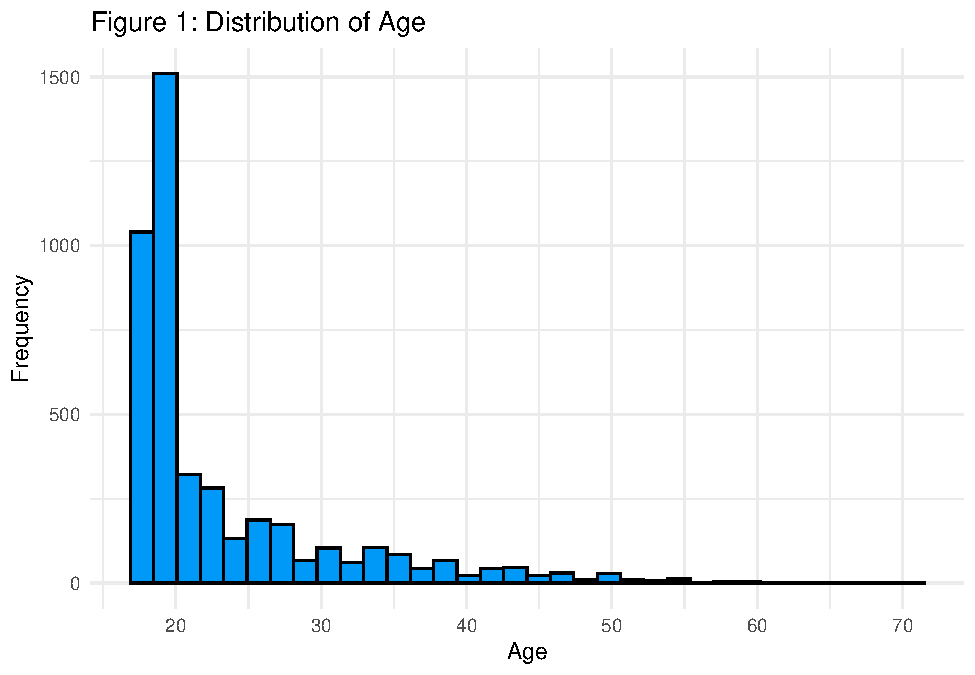
\includegraphics{finalproj_files/figure-latex/unnamed-chunk-6-1} \end{center}

\begin{table}

\caption{\label{tab:unnamed-chunk-6}Table 1: Summary Statistics - Age}
\centering
\begin{tabular}[t]{llllllll}
\toprule
Variable & N & Mean & Median & Min & 25% & 75% & Max\\
\midrule
Age & 4424 & 23 & 20 & 17 & 19 & 25 & 70\\
\bottomrule
\end{tabular}
\end{table}

The range of ages in the data lies between 17 and 70. Taking a look at
the summary statistics and distribution of values, we see that this
variable is heavily right skewed. It appears that 50\% of the
observations lie between 17-20 years old, with the highest frequency
being at 18 years old. This is nothing unusual, since most students
enroll in undergraduate degrees between these ages. The oldest
observation belonging to a 70 year old is not unusual either since many
adults choose to attend universities later on in their lives.

\hypertarget{nationality}{%
\subsubsection{Nationality}\label{nationality}}

\begin{table}

\caption{\label{tab:unnamed-chunk-7}Table 2: Nationality Frequency Table}
\centering
\begin{tabular}[t]{c|c}
\hline
Nationality Number & Frequency\\
\hline
Angolan & 2\\
\hline
Brazilian & 38\\
\hline
Cape Verdean & 13\\
\hline
Colombian & 1\\
\hline
Cuban & 1\\
\hline
Dutch & 1\\
\hline
English & 1\\
\hline
German & 2\\
\hline
Guinean & 5\\
\hline
Italian & 3\\
\hline
Lithuanian & 1\\
\hline
Mexican & 2\\
\hline
Moldova (Republic of) & 3\\
\hline
Mozambican & 2\\
\hline
Portuguese & 4314\\
\hline
Romanian & 2\\
\hline
Russian & 2\\
\hline
Santomean & 14\\
\hline
Spanish & 13\\
\hline
Turkish & 1\\
\hline
Ukrainian & 3\\
\hline
\end{tabular}
\end{table}

\begin{center}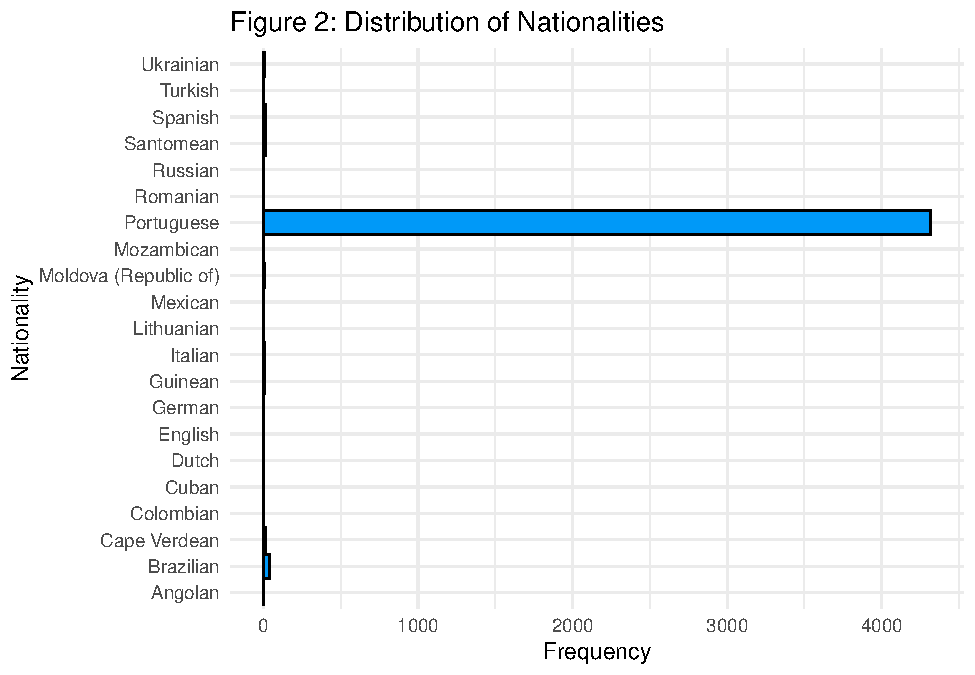
\includegraphics{finalproj_files/figure-latex/unnamed-chunk-7-1} \end{center}

There are a total of 21 nationalities amongst all observations in the
data. Looking at the distribution of nationalities in the data, we see
that almost all the observations belong to students of Portuguese
(Nationality \#1) descent. Since this data was collected from Portuguese
institutions, this is expected. There may be other reasons for such a
low concentration of observations with other nationalities such as
incomplete observations, etc. It is also important to take into account
that this may perhaps lead to non-generalizability of results.

\hypertarget{courseprogram}{%
\subsubsection{Course/Program}\label{courseprogram}}

\begin{table}

\caption{\label{tab:unnamed-chunk-8}Table 3: Course/Program Frequency Table}
\centering
\begin{tabular}[t]{c|c}
\hline
Program Number & Frequency\\
\hline
Advertising and Marketing Management & 268\\
\hline
Agronomy & 210\\
\hline
Animation and Multimedia Design & 215\\
\hline
Basic Education & 192\\
\hline
Biofuel Production Technologies & 12\\
\hline
Communication Design & 226\\
\hline
Equiniculture & 141\\
\hline
Informatics Engineering & 170\\
\hline
Journalism and Communication & 331\\
\hline
Management & 380\\
\hline
Management (evening attendance) & 268\\
\hline
Nursing & 766\\
\hline
Oral Hygiene & 86\\
\hline
Social Service & 355\\
\hline
Social Service (evening attendance) & 215\\
\hline
Tourism & 252\\
\hline
Veterinary Nursing & 337\\
\hline
\end{tabular}
\end{table}

\begin{center}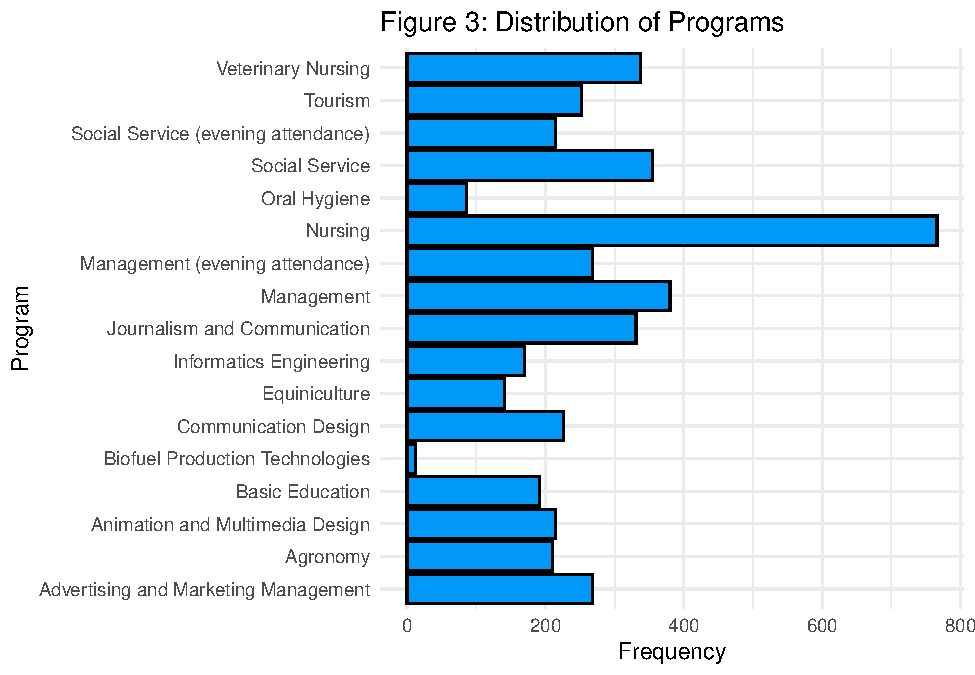
\includegraphics{finalproj_files/figure-latex/unnamed-chunk-8-1} \end{center}

There are a total of 17 programs of study amongst all observations. The
observations seem to be mostly evenly distributed among all programs,
except Biofuel Production Technologies (Program \#1) which has the least
number of observations (only 12) and Nursing (Program \#12) which has
the most number of observations (only 766).

\hypertarget{previous-qualification}{%
\subsubsection{Previous Qualification}\label{previous-qualification}}

\begin{table}

\caption{\label{tab:unnamed-chunk-9}Table 4: Previous Qualification Frequency Table}
\centering
\begin{tabular}[t]{c|c}
\hline
Previous Qualification Number & Frequency\\
\hline
10th year of schooling & 1\\
\hline
10th year of schooling—not completed & 2\\
\hline
11th year of schooling—not completed & 4\\
\hline
12th year of schooling—not completed & 11\\
\hline
Basic education 2nd cycle (6th/7th/8th year) or equivalent & 7\\
\hline
Basic education 3rd cycle (9th/10th/11th year) or equivalent & 162\\
\hline
Frequency of higher education & 16\\
\hline
Higher education—bachelor’s degree & 23\\
\hline
Higher education—degree & 126\\
\hline
Higher education—degree (1st cycle) & 40\\
\hline
Higher education—doctorate & 1\\
\hline
Higher education—master’s degree & 8\\
\hline
Higher education—master’s degree (2nd cycle) & 6\\
\hline
Other—11th year of schooling & 45\\
\hline
Professional higher technical course & 36\\
\hline
Secondary education & 3717\\
\hline
Technological specialization course & 219\\
\hline
\end{tabular}
\end{table}

\begin{center}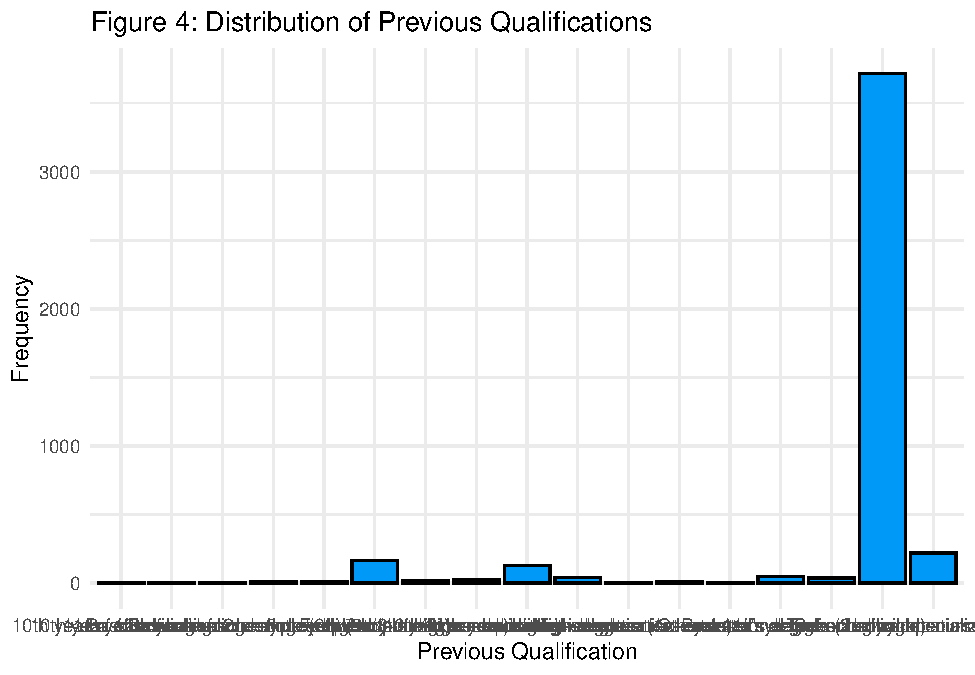
\includegraphics{finalproj_files/figure-latex/unnamed-chunk-9-1} \end{center}

There are 17 categories of previous qualifications listed in the
dataset. The most frequent observation is Secondary Education (Previous
qualification \#1). This is also expected since a large majority of
students come to universities to pursue undergraduate degrees after
completing high school/12th grade. Compared to Secondary Education, the
observations in the rest of the categories are minimal.

\hypertarget{mothers-qualification}{%
\subsubsection{Mother's Qualification}\label{mothers-qualification}}

\begin{table}

\caption{\label{tab:unnamed-chunk-10}Table 5: Mother's Qualification Frequency Table}
\centering
\begin{tabular}[t]{c|c}
\hline
Mother's Qualification Number & Frequency\\
\hline
10th Year of Schooling & 1\\
\hline
11th Year of Schooling—not completed & 3\\
\hline
12th Year of Schooling—not completed & 8\\
\hline
2nd cycle of the general high school course & 130\\
\hline
2nd year complementary high school course & 2\\
\hline
7th Year (Old) & 3\\
\hline
7th year of schooling & 3\\
\hline
8th year of schooling & 3\\
\hline
9th Year of Schooling—not completed & 3\\
\hline
Basic education 1st cycle (4th/5th year) or equivalent & 4\\
\hline
Basic Education 2nd Cycle (6th/7th/8th Year) or equivalent & 4\\
\hline
Basic Education 3rd Cycle (9th/10th/11th Year) or Equivalent & 1\\
\hline
Can read without having a 4th year of schooling & 6\\
\hline
Cannot read or write & 9\\
\hline
Complementary High School Course & 1\\
\hline
Complementary High School Course—not concluded & 3\\
\hline
Frequency of Higher Education & 4\\
\hline
General commerce course & 953\\
\hline
General Course of Administration and Commerce & 1009\\
\hline
Higher Education—bachelor’s degree & 83\\
\hline
Higher Education—degree & 438\\
\hline
Higher Education—doctorate & 21\\
\hline
Higher Education—master’s degree & 49\\
\hline
Other—11th Year of Schooling & 42\\
\hline
Secondary Education—12th Year of Schooling or Equivalent & 1069\\
\hline
Supplementary Accounting and Administration & 562\\
\hline
Technical-professional course & 1\\
\hline
Technological specialization course & 1\\
\hline
Unknown & 8\\
\hline
\end{tabular}
\end{table}

\begin{center}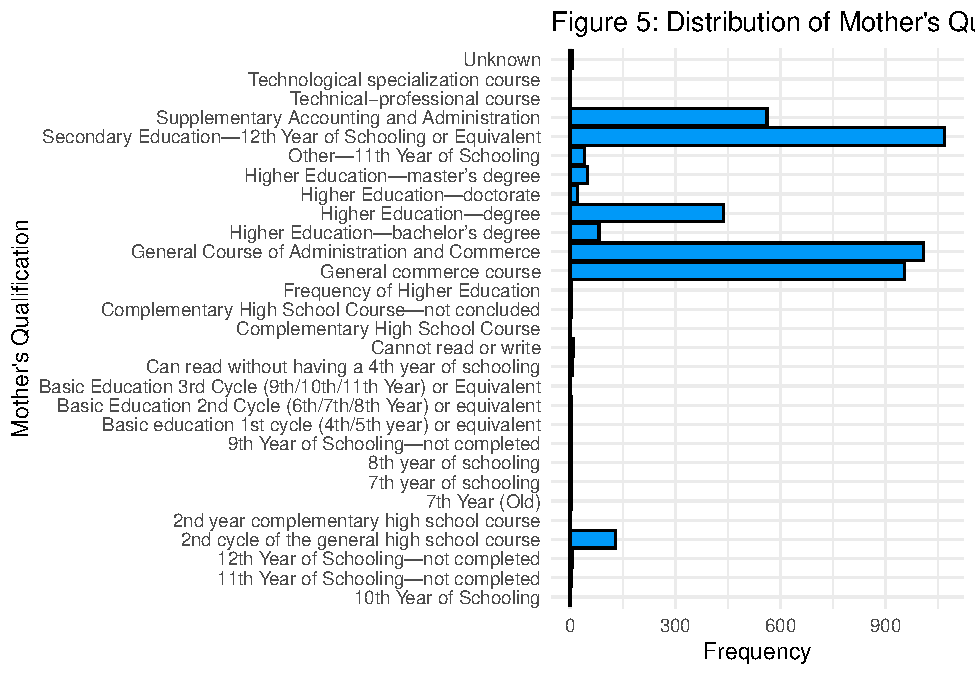
\includegraphics{finalproj_files/figure-latex/unnamed-chunk-10-1} \end{center}

For this variable, there are 34 defined categories in the documentation,
but only 29 categories were found among all observations. Since all of
the categories in this variable are numbered from 1-29, this doesn't
indicate an error in the data. It may perhaps just be because both
mother's and father's qualification values were defined in one table
since both these variables have the first 29 values in common and the
last five are additional in the latter variable. There appear to be
three categories that these observations are primarily distributed into.
Ordered from highest frequency to lowest, these are Secondary
Education---12th Year of Schooling or Equivalent (Program \#1), General
Course of Administration and Commerce, and General commerce course. It
appears that a large number of students in this dataset have mothers who
took some form of commerce course. This may indicate a trend or may have
some correlation with admission or dropout rates that may need to be
further explored.

\hypertarget{fathers-qualification}{%
\subsubsection{Father's Qualification}\label{fathers-qualification}}

\begin{table}

\caption{\label{tab:unnamed-chunk-11}Table 6: Father's Qualification Frequency Table}
\centering
\begin{tabular}[t]{c|c}
\hline
Father's Qualification Number & Frequency\\
\hline
10th Year of Schooling & 4\\
\hline
11th Year of Schooling—not completed & 2\\
\hline
12th Year of Schooling—not completed & 5\\
\hline
2nd cycle of the general high school course & 1\\
\hline
2nd year complementary high school course & 1\\
\hline
7th Year (Old) & 10\\
\hline
7th year of schooling & 2\\
\hline
8th year of schooling & 4\\
\hline
9th Year of Schooling—not completed & 3\\
\hline
Basic education 1st cycle (4th/5th year) or equivalent & 1209\\
\hline
Basic Education 2nd Cycle (6th/7th/8th Year) or equivalent & 702\\
\hline
Basic Education 3rd Cycle (9th/10th/11th Year) or Equivalent & 968\\
\hline
Can read without having a 4th year of schooling & 8\\
\hline
Cannot read or write & 2\\
\hline
Complementary High School Course & 1\\
\hline
Complementary High School Course—not concluded & 1\\
\hline
Frequency of Higher Education & 2\\
\hline
General commerce course & 1\\
\hline
General Course of Administration and Commerce & 1\\
\hline
Higher Education—bachelor’s degree & 68\\
\hline
Higher Education—degree & 282\\
\hline
Higher education—degree (1st cycle) & 5\\
\hline
Higher Education—doctorate & 18\\
\hline
Higher Education—doctorate (3rd cycle) & 1\\
\hline
Higher Education—master’s degree & 39\\
\hline
Higher Education—master’s degree (2nd cycle) & 2\\
\hline
Other—11th Year of Schooling & 38\\
\hline
Professional higher technical course & 1\\
\hline
Secondary Education—12th Year of Schooling or Equivalent & 904\\
\hline
Specialized higher studies course & 2\\
\hline
Supplementary Accounting and Administration & 1\\
\hline
Technical-professional course & 4\\
\hline
Technological specialization course & 20\\
\hline
Unknown & 112\\
\hline
\end{tabular}
\end{table}

\begin{center}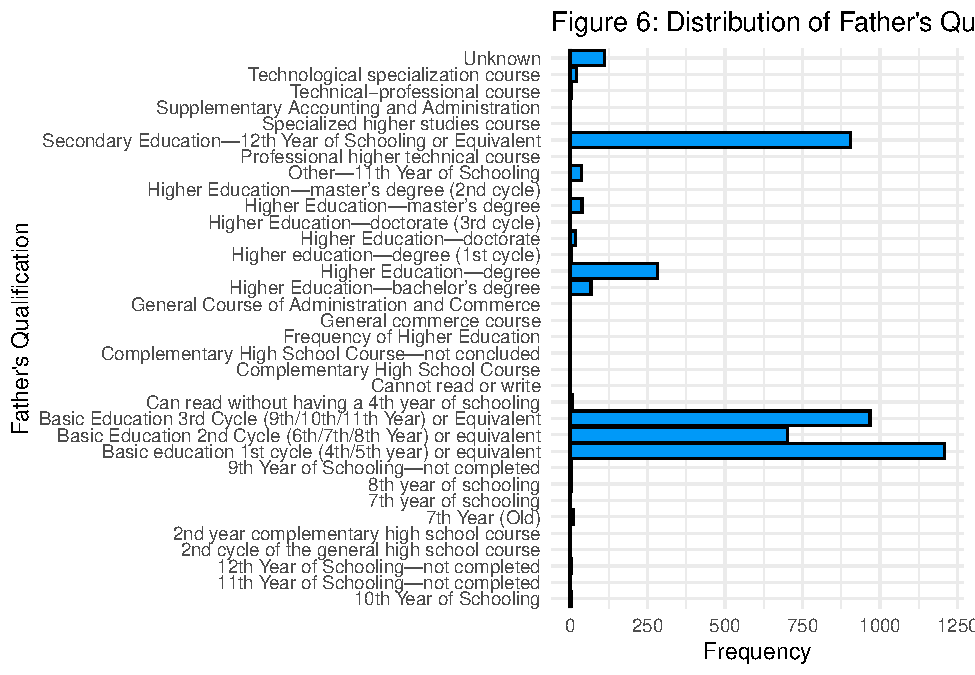
\includegraphics{finalproj_files/figure-latex/unnamed-chunk-11-1} \end{center}

For this variable, there are 34 defined categories in the documentation,
and all of them were found in the dataset. Similar to the mother's
qualification variable, the observations in the dataset seem to be
primarily distributed into three categories - Basic education 1st cycle
(4th/5th year) or equivalent, Basic Education 3rd Cycle (9th/10th/11th
Year) or Equivalent, Secondary Education---12th Year of Schooling or
Equivalent. This may indicate that a large number of students may be
first generation university students.

For both the Mother's Qualification and Father's Qualification
variables, there is a certain category called ``Unknown'' in which a
small fraction of observations lie (approximately 120 observations).
This is a very small number of observations as compared to the total
number of observations in the dataset and can be removed. However, this
variable may indicate other information, such as the student not
knowing/having ever met this parent and thus not knowing their
qualifications. Due to this, we chose to leave all observations with
this value in the dataset.

\hypertarget{gender}{%
\subsubsection{Gender}\label{gender}}

\begin{table}

\caption{\label{tab:unnamed-chunk-12}Table 7: Gender Frequency Table}
\centering
\begin{tabular}[t]{c|c}
\hline
Gender & Frequency\\
\hline
Female & 2868\\
\hline
Male & 1556\\
\hline
\end{tabular}
\end{table}

Looking at the frequency table, we see that there is a greater number of
observations that belong to students who are female as opposed to those
that are male. In fact, there are almost twice the number of females as
opposed to males in this dataset. This may skew results in an
undesirable manner; the full effect of this needs to be investigated
further.

\hypertarget{unemployment-rate}{%
\subsubsection{Unemployment Rate}\label{unemployment-rate}}

\begin{center}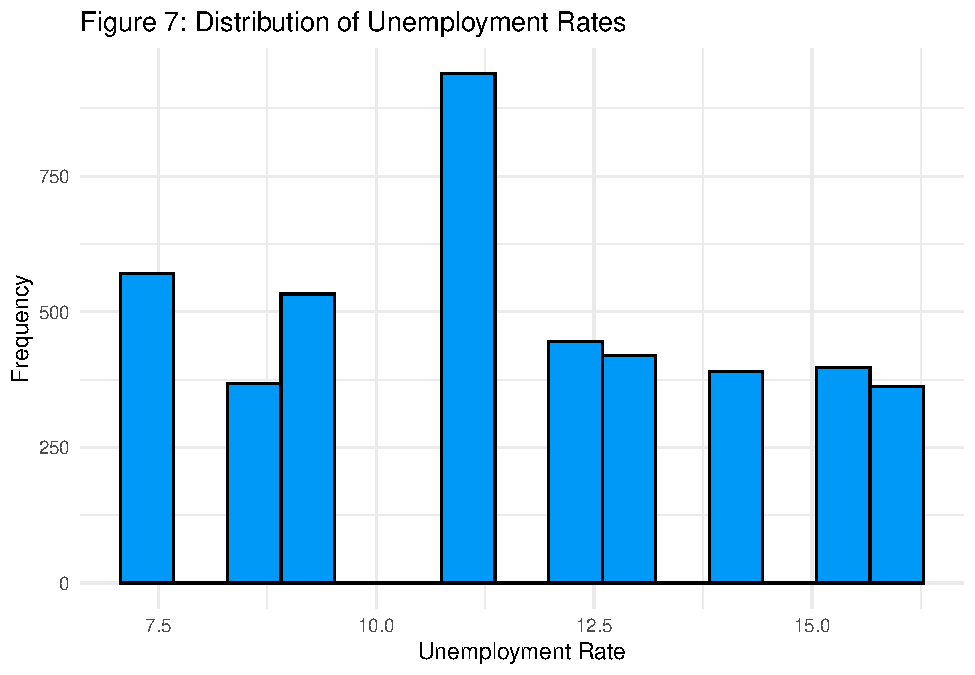
\includegraphics{finalproj_files/figure-latex/unnamed-chunk-13-1} \end{center}

\begin{table}

\caption{\label{tab:unnamed-chunk-13}Table 8: Summary Statistics - Unemployment Rate}
\centering
\begin{tabular}[t]{llllllll}
\toprule
Variable & N & Mean & Median & Min & 25% & 75% & Max\\
\midrule
Unemp_rate & 4424 & 12 & 11 & 7.6 & 9.4 & 14 & 16\\
\bottomrule
\end{tabular}
\end{table}

The summary statistics and histogram tell us that the unemployment rates
vary from 7.6\% to 16.2\% over the years, which is in accordance with
secondary sources of historical data which looked at rates between 2008
and 2019. There seems to be a high concentration of values around the
11\% mark, which may indicate that a large number of observations may
have been from a particular year/time where the unemployment rate
hovered around this mark. This may potentially skew results.

\hypertarget{target}{%
\subsubsection{Target}\label{target}}

\begin{center}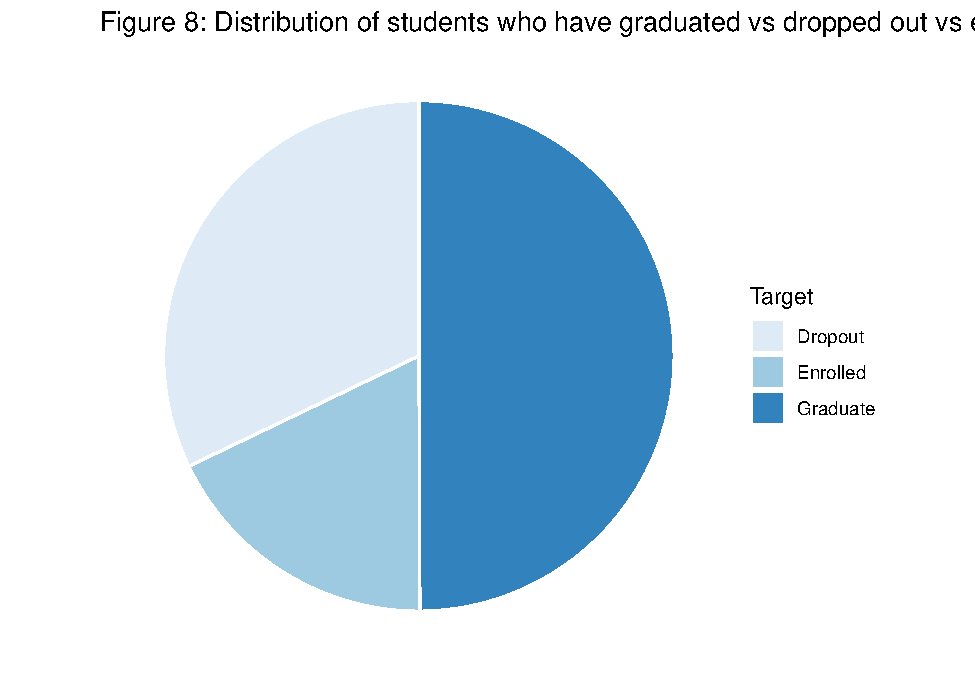
\includegraphics{finalproj_files/figure-latex/unnamed-chunk-14-1} \end{center}

The Target variable consists of three categories - ``Dropped'',
``Enrolled'', and Graduate''. Taking a look at this pie chart, we see
that around half the students in this dataset graduated from university,
one third of the students dropped out, and one sixth are still enrolled
in university at the time of data collection (these are perhaps students
who enrolled university in the later years of data collection (ex: 2018,
2019).

\hypertarget{life-expectancy}{%
\subsubsection{Life Expectancy}\label{life-expectancy}}

\begin{center}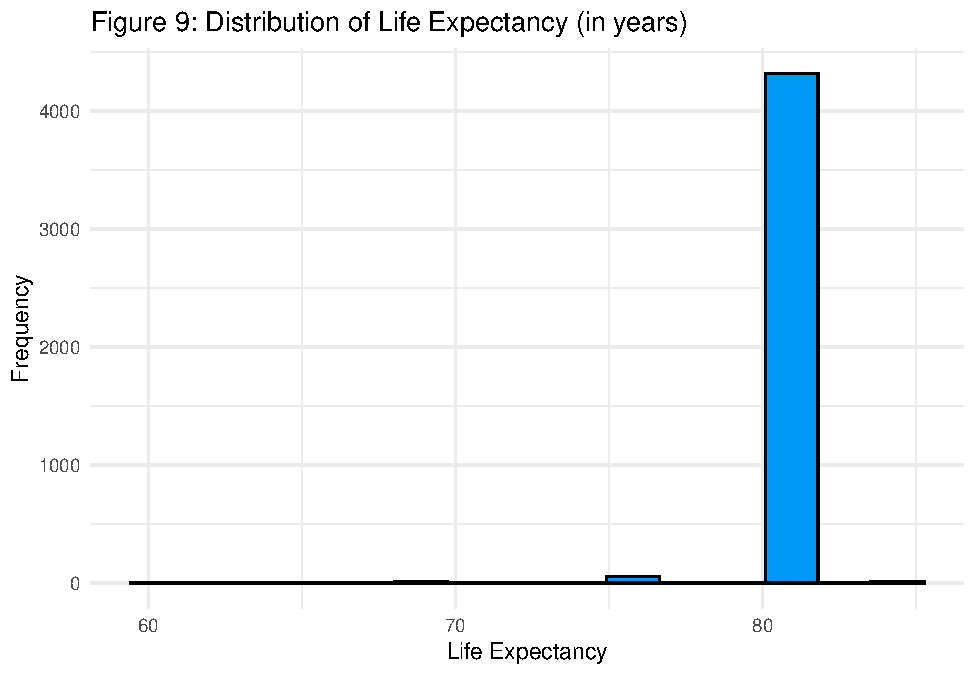
\includegraphics{finalproj_files/figure-latex/unnamed-chunk-15-1} \end{center}

\begin{table}

\caption{\label{tab:unnamed-chunk-15}Table 9: Summary Statistics - Life Expectancy}
\centering
\begin{tabular}[t]{llllllll}
\toprule
Variable & N & Mean & Median & Min & 25% & 75% & Max\\
\midrule
Life_expectancy & 4424 & 81 & 82 & 60 & 82 & 82 & 84\\
\bottomrule
\end{tabular}
\end{table}

Finally, taking a look at the summary statistics and distribution of the
life expectancy variable, we see that almost all the observations are at
around the 81 (years) mark. This follows from the fact that a majority
of observations are from students of Portuguese nationality - since we
assigned these values based on nationality, it was bound that the
distribution would be skewed as such. Due to this, it is unclear how
useful this variable will be in prediction.

\hypertarget{initial-logistic-regression-model}{%
\subsection{Initial Logistic Regression
Model}\label{initial-logistic-regression-model}}

\begin{verbatim}
## Warning in predict.lm(object, newdata, se.fit, scale = 1, type = if (type == :
## prediction from a rank-deficient fit may be misleading
\end{verbatim}

\begin{table}
\centering
\begin{tabular}[t]{lc}
\toprule
  & Initial Logistic Regression Model\\
\midrule
(Intercept) & \num{-1.068900e+16}\\
 & (\num{106772227.055})\\
NationalityBrazilian & \num{3.029966e+14}\\
 & (\num{48936808.475})\\
NationalityCape Verdean & \num{5.974871e+14}\\
 & (\num{51263863.027})\\
NationalityColombian & \num{-3.842659e+15}\\
 & (\num{82505836.780})\\
NationalityCuban & \num{3.043001e+15}\\
 & (\num{82819508.241})\\
NationalityDutch & \num{4.435730e+15}\\
 & (\num{82427011.509})\\
NationalityEnglish & \num{3.563298e+15}\\
 & (\num{82543924.227})\\
NationalityGerman & \num{4.610831e+15}\\
 & (\num{67439062.592})\\
NationalityGuinean & \num{2.159503e+15}\\
 & (\num{56389425.456})\\
NationalityItalian & \num{3.724116e+15}\\
 & (\num{62102053.327})\\
NationalityLithuanian & \num{-4.028895e+15}\\
 & (\num{82500002.830})\\
NationalityMexican & \num{-1.022669e+15}\\
 & (\num{67610244.923})\\
NationalityMoldova (Republic of) & \num{-4.914652e+14}\\
 & (\num{62827769.673})\\
NationalityMozambican & \num{2.102280e+15}\\
 & (\num{67860486.448})\\
NationalityPortuguese & \num{3.105968e+14}\\
 & (\num{47700494.025})\\
NationalityRomanian & \num{2.369894e+15}\\
 & (\num{67409112.840})\\
NationalityRussian & \num{7.794034e+14}\\
 & (\num{67402090.607})\\
NationalitySantomean & \num{1.688247e+15}\\
 & (\num{51010948.876})\\
NationalitySpanish & \num{8.844869e+14}\\
 & (\num{51343411.075})\\
NationalityTurkish & \num{5.696228e+15}\\
 & (\num{82572034.979})\\
NationalityUkrainian & \num{-4.155361e+14}\\
 & (\num{61690889.040})\\
ProgramAgronomy & \num{7.457329e+13}\\
 & (\num{6619641.115})\\
ProgramAnimation and Multimedia Design & \num{-3.418493e+14}\\
 & (\num{6235544.122})\\
ProgramBasic Education & \num{-6.781356e+14}\\
 & (\num{6484991.127})\\
ProgramBiofuel Production Technologies & \num{-2.431709e+15}\\
 & (\num{20018566.749})\\
ProgramCommunication Design & \num{1.548294e+15}\\
 & (\num{6131926.091})\\
ProgramEquiniculture & \num{-1.411009e+15}\\
 & (\num{7209508.959})\\
ProgramInformatics Engineering & \num{-1.463131e+15}\\
 & (\num{6796702.637})\\
ProgramJournalism and Communication & \num{-1.285576e+15}\\
 & (\num{5608884.616})\\
ProgramManagement & \num{2.075431e+14}\\
 & (\num{5423320.895})\\
ProgramManagement (evening attendance) & \num{4.403783e+14}\\
 & (\num{6148857.872})\\
ProgramNursing & \num{8.521410e+14}\\
 & (\num{4875059.249})\\
ProgramOral Hygiene & \num{-9.873897e+14}\\
 & (\num{8519703.576})\\
ProgramSocial Service & \num{2.953534e+14}\\
 & (\num{5555713.231})\\
ProgramSocial Service (evening attendance) & \num{1.167612e+15}\\
 & (\num{6598322.710})\\
ProgramTourism & \num{-2.292741e+14}\\
 & (\num{5942450.784})\\
ProgramVeterinary Nursing & \num{-2.366876e+14}\\
 & (\num{5676472.386})\\
Prev\_quali10th year of schooling—not completed & \num{4.538100e+15}\\
 & (\num{82412875.003})\\
Prev\_quali11th year of schooling—not completed & \num{4.926899e+15}\\
 & (\num{75520192.687})\\
Prev\_quali12th year of schooling—not completed & \num{2.264829e+15}\\
 & (\num{70504220.504})\\
Prev\_qualiBasic education 2nd cycle (6th/7th/8th year) or equivalent & \num{5.377821e+15}\\
 & (\num{72165343.072})\\
Prev\_qualiBasic education 3rd cycle (9th/10th/11th year) or equivalent & \num{4.478615e+15}\\
 & (\num{67724385.310})\\
Prev\_qualiFrequency of higher education & \num{6.128150e+15}\\
 & (\num{69602725.423})\\
Prev\_qualiHigher education—bachelor’s degree & \num{3.730218e+15}\\
 & (\num{68990993.308})\\
Prev\_qualiHigher education—degree & \num{4.512438e+15}\\
 & (\num{67784151.936})\\
Prev\_qualiHigher education—degree (1st cycle) & \num{4.555584e+15}\\
 & (\num{68379362.459})\\
Prev\_qualiHigher education—doctorate & \num{3.986846e+15}\\
 & (\num{95359605.213})\\
Prev\_qualiHigher education—master’s degree & \num{5.046443e+15}\\
 & (\num{71689846.584})\\
Prev\_qualiHigher education—master’s degree (2nd cycle) & \num{4.719852e+15}\\
 & (\num{73106234.914})\\
Prev\_qualiOther—11th year of schooling & \num{4.842770e+15}\\
 & (\num{68210298.317})\\
Prev\_qualiProfessional higher technical course & \num{5.624397e+15}\\
 & (\num{68513318.771})\\
Prev\_qualiSecondary education & \num{5.143640e+15}\\
 & (\num{67549635.696})\\
Prev\_qualiTechnological specialization course & \num{4.433850e+15}\\
 & (\num{67724187.033})\\
Mom\_quali11th Year of Schooling—not completed & \num{9.291148e+15}\\
 & (\num{88672946.973})\\
Mom\_quali12th Year of Schooling—not completed & \num{7.225029e+15}\\
 & (\num{81016819.556})\\
Mom\_quali2nd cycle of the general high school course & \num{6.904755e+15}\\
 & (\num{77917978.063})\\
Mom\_quali2nd year complementary high school course & \num{6.618557e+15}\\
 & (\num{85055018.042})\\
Mom\_quali7th Year (Old) & \num{7.918266e+15}\\
 & (\num{87303188.736})\\
Mom\_quali7th year of schooling & \num{7.518655e+15}\\
 & (\num{86436042.670})\\
Mom\_quali8th year of schooling & \num{5.621763e+15}\\
 & (\num{81893724.082})\\
Mom\_quali9th Year of Schooling—not completed & \num{1.109754e+16}\\
 & (\num{102482859.502})\\
Mom\_qualiBasic education 1st cycle (4th/5th year) or equivalent & \num{8.702151e+15}\\
 & (\num{84577029.878})\\
Mom\_qualiBasic Education 2nd Cycle (6th/7th/8th Year) or equivalent & \num{7.365706e+15}\\
 & (\num{84817431.516})\\
Mom\_qualiBasic Education 3rd Cycle (9th/10th/11th Year) or Equivalent & \num{7.049332e+15}\\
 & (\num{112910389.006})\\
Mom\_qualiCan read without having a 4th year of schooling & \num{9.365471e+15}\\
 & (\num{81971780.498})\\
Mom\_qualiCannot read or write & \num{8.459948e+15}\\
 & (\num{80807850.133})\\
Mom\_qualiComplementary High School Course & \num{1.184828e+16}\\
 & (\num{112925443.135})\\
Mom\_qualiComplementary High School Course—not concluded & \num{9.182546e+15}\\
 & (\num{88541423.240})\\
Mom\_qualiFrequency of Higher Education & \num{1.025663e+16}\\
 & (\num{89957564.251})\\
Mom\_qualiGeneral commerce course & \num{7.685738e+15}\\
 & (\num{77215850.477})\\
Mom\_qualiGeneral Course of Administration and Commerce & \num{8.049275e+15}\\
 & (\num{77239015.720})\\
Mom\_qualiHigher Education—bachelor’s degree & \num{8.455323e+15}\\
 & (\num{77569104.227})\\
Mom\_qualiHigher Education—degree & \num{7.526287e+15}\\
 & (\num{77275764.107})\\
Mom\_qualiHigher Education—doctorate & \num{7.981093e+15}\\
 & (\num{78803530.246})\\
Mom\_qualiHigher Education—master’s degree & \num{8.887059e+15}\\
 & (\num{77829940.338})\\
Mom\_qualiOther—11th Year of Schooling & \num{6.985698e+15}\\
 & (\num{77921714.550})\\
Mom\_qualiSecondary Education—12th Year of Schooling or Equivalent & \num{7.595323e+15}\\
 & (\num{77203351.230})\\
Mom\_qualiSupplementary Accounting and Administration & \num{8.006597e+15}\\
 & (\num{77205649.986})\\
Mom\_qualiTechnical-professional course & \num{3.489703e+15}\\
 & (\num{102618475.203})\\
Mom\_qualiTechnological specialization course & \num{1.039924e+16}\\
 & (\num{108502481.460})\\
Mom\_qualiUnknown & \num{6.291367e+15}\\
 & (\num{81191012.485})\\
Dad\_quali11th Year of Schooling—not completed & \num{-7.986395e+15}\\
 & (\num{69589931.267})\\
Dad\_quali12th Year of Schooling—not completed & \num{-7.253411e+14}\\
 & (\num{48808628.487})\\
Dad\_quali2nd cycle of the general high school course & \num{-4.196792e+15}\\
 & (\num{90218660.760})\\
Dad\_quali2nd year complementary high school course & \num{-5.412307e+15}\\
 & (\num{77378095.007})\\
Dad\_quali7th Year (Old) & \num{-2.331520e+15}\\
 & (\num{43072504.995})\\
Dad\_quali7th year of schooling & \num{5.108896e+13}\\
 & (\num{61197533.751})\\
Dad\_quali8th year of schooling & \num{-1.856225e+15}\\
 & (\num{61068214.418})\\
Dad\_quali9th Year of Schooling—not completed & \num{-4.822924e+15}\\
 & (\num{54691605.122})\\
Dad\_qualiBasic education 1st cycle (4th/5th year) or equivalent & \num{-1.501889e+15}\\
 & (\num{38103253.083})\\
Dad\_qualiBasic Education 2nd Cycle (6th/7th/8th Year) or equivalent & \num{-1.571931e+15}\\
 & (\num{38136890.464})\\
Dad\_qualiBasic Education 3rd Cycle (9th/10th/11th Year) or Equivalent & \num{-1.733481e+15}\\
 & (\num{38123453.231})\\
Dad\_qualiCan read without having a 4th year of schooling & \num{-1.015358e+15}\\
 & (\num{44165767.459})\\
Dad\_qualiCannot read or write & \num{-6.918090e+15}\\
 & (\num{91177220.251})\\
Dad\_qualiComplementary High School Course & \num{-1.047302e+15}\\
 & (\num{77531152.855})\\
Dad\_qualiComplementary High School Course—not concluded & \num{-7.539839e+15}\\
 & (\num{77432630.898})\\
Dad\_qualiFrequency of Higher Education & \num{-4.111893e+15}\\
 & (\num{64944510.478})\\
Dad\_qualiGeneral Course of Administration and Commerce & \num{-6.020610e+15}\\
 & (\num{77337168.040})\\
Dad\_qualiHigher Education—bachelor’s degree & \num{-1.414260e+15}\\
 & (\num{38994937.318})\\
Dad\_qualiHigher Education—degree & \num{-1.596297e+15}\\
 & (\num{38328204.719})\\
Dad\_qualiHigher education—degree (1st cycle) & \num{-3.517365e+15}\\
 & (\num{51908252.769})\\
Dad\_qualiHigher Education—doctorate & \num{-2.127172e+15}\\
 & (\num{41617599.361})\\
Dad\_qualiHigher Education—doctorate (3rd cycle) & \num{-2.248718e+15}\\
 & (\num{77266622.972})\\
Dad\_qualiHigher Education—master’s degree & \num{-1.381535e+15}\\
 & (\num{39706382.343})\\
Dad\_qualiHigher Education—master’s degree (2nd cycle) & \num{2.482638e+15}\\
 & (\num{62669299.801})\\
Dad\_qualiOther—11th Year of Schooling & \num{-1.376462e+15}\\
 & (\num{39743629.169})\\
Dad\_qualiProfessional higher technical course & \num{3.821611e+15}\\
 & (\num{77241235.771})\\
Dad\_qualiSecondary Education—12th Year of Schooling or Equivalent & \num{-1.451970e+15}\\
 & (\num{38137698.181})\\
Dad\_qualiSpecialized higher studies course & \num{-9.890083e+14}\\
 & (\num{61470299.426})\\
Dad\_qualiSupplementary Accounting and Administration & \num{-7.708756e+14}\\
 & (\num{77242590.333})\\
Dad\_qualiTechnical-professional course & \num{-5.891158e+15}\\
 & (\num{53794320.709})\\
Dad\_qualiTechnological specialization course & \num{-1.947193e+15}\\
 & (\num{41320883.516})\\
Dad\_qualiUnknown & \num{-1.515737e+15}\\
 & (\num{39682138.974})\\
GenderMale & \num{-1.889799e+14}\\
 & (\num{2409561.225})\\
Age & \num{-3.505464e+13}\\
 & (\num{188585.902})\\
Unemp\_rate & \num{5.425617e+13}\\
 & (\num{417489.100})\\
\midrule
Num.Obs. & \num{4424}\\
AIC & \\
BIC & \\
Log.Lik. & \\
RMSE & \num{0.57}\\
\bottomrule
\end{tabular}
\end{table}

Fitting an initial naive logistic regression model in order to explore
the formulated question further, we see that some variables seem to be
having significant effects on the response variable whereas others seem
to not have a significant effect at all. The RMSE value calculated is
also very low, implying that the model is not very capable of prediction
in its current form. In order to decipher which factors have the most
impact on dropout rates and will help us build a model that is capable
of accurate predictions, we can use stepwise logistic regression.

Another approach could be the use of other machine learning models. We
can fit other models (such as xgboost, random forests, etc.) that help
to better describe the data and make more accurate predictions. This
approach must be explored further in this project.

At this point, we cannot say whether we can predict whether a student
will drop out of university or not based on the prior mentioned
socioeconomic factors. Further modeling and analysis must be done in
order to answer this question concretely.

\hypertarget{description-of-modeling}{%
\section{Description of Modeling}\label{description-of-modeling}}

Building upon our preliminary findings, we decided to make use of three
machine learning models in order to best answer our question. These
models are Gradient Boosting, Random Forest, and XGBOOST, which we
evaluated on accuracy, MSE, and misclassification error. These models
were chosen as they are popular machine learning models that are
especially used for classification tasks. Before these models were
trained, the data was split up into training and testing data, where
80\% of the data was devoted to training the model, and 20\% of the data
was devoted to testing.

After tuning the hyperparameters, the gradient boosting model that gave
us the best results was constructed with 10-fold cross validation, 5000
trees, shrinkage rate of 0.001, and interaction depth of 2. The optimal
random forest model was selected with a complexity parameter of
(INSERT). In order to tune the hyperparameters for the XGBOOST model, we
performed a grid search with 10-fold cross validation, maximum tree
depths of 1,3,5,7,9, and 11, 50 to 500 trees, and learning rates of 0.5,
.3, .1, .01, .001, and 0.0001. The final values used for the model were
500 trees, maximum tree depth of 3, learning rate of 0.01, and default
gamma value of 0.

These models were then used to generate predictions using the reserved
test dataset, and were evaluated on three main metrics - accuracy,
misclassification error, MSE.

\begin{verbatim}
## Warning: package 'gbm' was built under R version 4.2.3
\end{verbatim}

\begin{verbatim}
## Warning: package 'caret' was built under R version 4.2.3
\end{verbatim}

\begin{verbatim}
## Warning: Setting `distribution = "multinomial"` is ill-advised as it is
## currently broken. It exists only for backwards compatibility. Use at your own
## risk.

## Warning: Setting `distribution = "multinomial"` is ill-advised as it is
## currently broken. It exists only for backwards compatibility. Use at your own
## risk.
\end{verbatim}

\begin{verbatim}
## [1] 1.027861
\end{verbatim}

\hypertarget{results}{%
\section{Results}\label{results}}

\hypertarget{gradient-boosting}{%
\subsubsection{Gradient Boosting}\label{gradient-boosting}}

\begin{table}

\caption{\label{tab:unnamed-chunk-22}Relative Influence plot (GBM)}
\centering
\begin{tabular}[t]{l|c|c}
\hline
  & Variable & Relative Influence\\
\hline
Program & Program & 39.5135194\\
\hline
Age & Age & 23.2580573\\
\hline
Mom\_quali & Mom\_quali & 11.6628285\\
\hline
Dad\_quali & Dad\_quali & 11.0475296\\
\hline
Gender & Gender & 5.4654287\\
\hline
Prev\_quali & Prev\_quali & 4.9838727\\
\hline
Nationality & Nationality & 2.2732446\\
\hline
Unemp\_rate & Unemp\_rate & 1.7931935\\
\hline
Life\_expectancy & Life\_expectancy & 0.0023256\\
\hline
\end{tabular}
\end{table}

\begin{table}

\caption{\label{tab:unnamed-chunk-22}Gradient Boosting Evaluation Metrics}
\centering
\begin{tabular}[t]{c|c|c}
\hline
Accuracy & Misclasssification Error & MSE\\
\hline
0.6069 & 0.3930723 & 1.027861\\
\hline
\end{tabular}
\end{table}

The Gradient Boosting model achieved an accuracy of 0.6069, which means
it correctly predicts the class of the response variable 60.69\% of the
time. a misclassification error of 0.3930723, and a mean squared error
of 1.027861. The misclassification error suggests that about 39\% of the
predictions made by the were incorrect, while the MSE suggests that the
model's predictions were on average 1.027861 units away from the true
values.

As for variable importance, we see that the variables Program
(39.5135194) and Age (23.2580573) seem to have the highest influence on
the model, with Life\_expectancy (0.0023256) having almost negligible
influence.

\hypertarget{random-forest}{%
\subsubsection{Random Forest}\label{random-forest}}

\begin{center}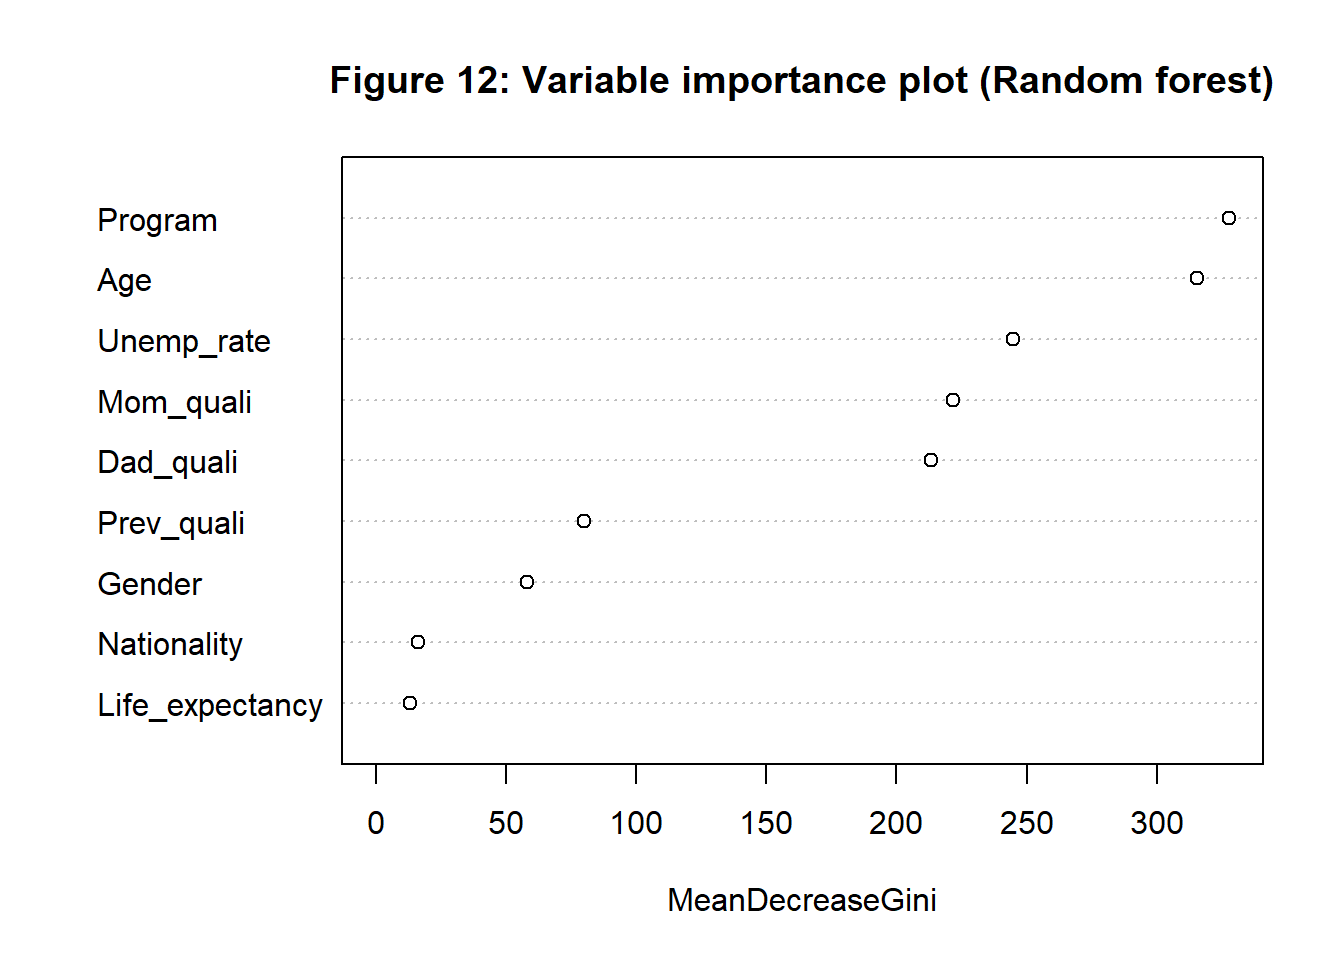
\includegraphics{finalproj_files/figure-latex/unnamed-chunk-23-1} \end{center}

\begin{table}

\caption{\label{tab:unnamed-chunk-23}Random Forest Evaluation Metrics}
\centering
\begin{tabular}[t]{c|c|c}
\hline
Accuracy & Misclasssification Error & MSE\\
\hline
0.5791 & 0.4209337 & 1.15738\\
\hline
\end{tabular}
\end{table}

The Random Forest classification model achieved an accuracy of 0.5791, a
misclassification error of 0.4209, and a mean squared error of 1.1574.
The model had a moderate accuracy and a relatively higher
misclassification error, indicating that it had some difficulty in
classifying the response variable correctly.

In terms of variable importance for the random forest model, we observe
similar behavior as we did for GBM. Taking a look at the variable
importance plot, we see that Program and Age have the highest importance
in the model, and Life\_expectancy and Nationality have the lowest.

\hypertarget{xgboost}{%
\subsubsection{XGBOOST}\label{xgboost}}

\begin{center}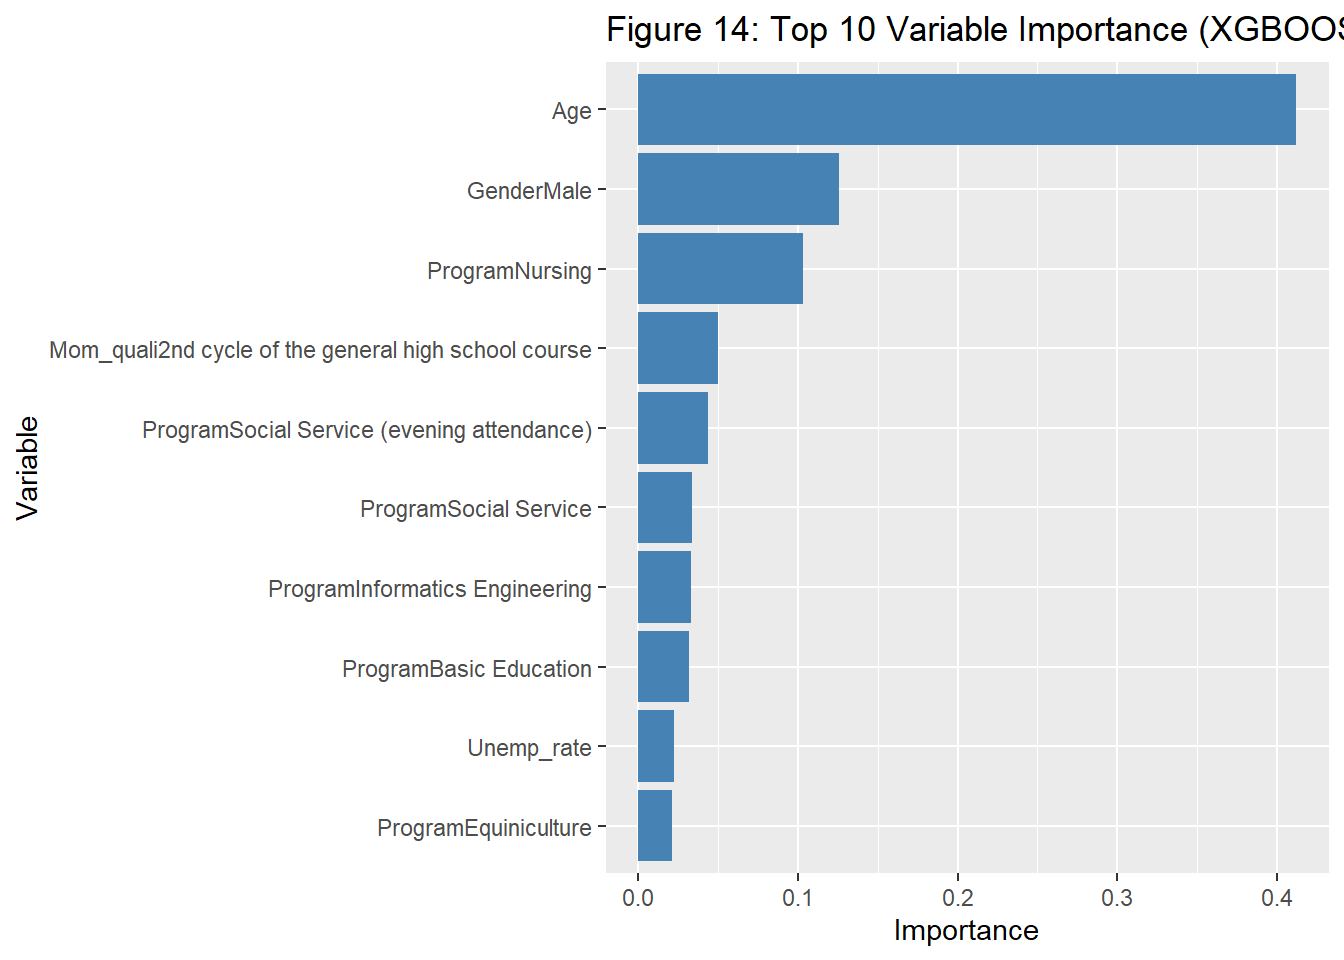
\includegraphics{finalproj_files/figure-latex/unnamed-chunk-24-1} \end{center}

\begin{table}

\caption{\label{tab:unnamed-chunk-24}XGBOOST Evaluation Metrics}
\centering
\begin{tabular}[t]{c|c|c}
\hline
Accuracy & Misclasssification Error & MSE\\
\hline
0.3133 & 0.686747 & 0.7567771\\
\hline
\end{tabular}
\end{table}

Based on the XGBoost classification model results, the accuracy is
0.3133 which indicates that the model is not performing well in
predicting the correct label. The misclassification error is high at
0.686747, indicating that a significant proportion of the predictions
are incorrect. The MSE is 0.7567771, indicating that the model's
predicted values differ significantly from the actual values. Although
the MSE is lower than that of GBM and Random Forest, the XGBoost model
needs improvement in terms of accuracy and misclassification error.

The variable importance plot generated measures the importance of each
category of each variable. This generated a very messy plot with many
variables that had negligible importance on the model. In order to
display the results that mattered most for this analysis, we filtered
down the plot so as to display only the top 10 most important variables.
We see that Age, Gender with the category Male, and Program with the
category Nursing seem to be the most important variables to this model,
with Age being the most important. This is very interesting, since the
variables that have the most influence in this model are slightly
different from those found in the plots for GBM and Random Forest
models. For example, Age is the most influential in this model, whereas
Program was the most influential in the others. The importance of the
rest of the variables in this model is less than 0.05.

\hypertarget{conclusion}{%
\section{Conclusion}\label{conclusion}}

Based on the results from the above models, we can see that the GBM
model outperforms the random forest and XGBOOST models in almost all the
metrics we are evaluating them against. The XGBOOST model has a lower
MSE than the GBM model, however, this might be due to the magnitude of
errors made by the model being small, even though it has misclassified a
large number of observations. In terms of the particular question we are
trying to answer, classifying the observations correctly seems to be
more important than the magnitude of error the model missed the
classification by. Hence, considering the given dataset, variables, and
models the GBM model seems to be the most appropriate model to use to
answer our research question.

As for answering the question, we can say that we can predict with 60\%
accuracy whether a student will drop out of an undergraduate degree
program, remain enrolled, or graduate based on factors such as gender,
unemployment rates, nationality, 2019 life expectancy (based on
nationality), previous qualification, mother's and father's
qualification, and program of study. This is not a very good accuracy,
implying that the model does not do a good job at prediction.

\hypertarget{limitations}{%
\subsubsection{Limitations}\label{limitations}}

There are many limitations to the project that may have affected results
and may also affect future analyses. We wish to address these in the
following section. We noticed that many of the variables used in these
models have little to no influence/importance on the models. Removing
these variables and/or adding more influential variables that are better
associated with the response variable may greatly impact the prediction
quality of the models. However, this may change the scope of the
research question, which is why this avenue was not explored. Since we
do not have a year variable, it is unclear how the varying trends in
social and economic factors through the years impacted our results and
predictions. In addition to this, almost all of the observations in the
dataset come from Portuguese nationals which may lead to our results and
predictions being hard to generalize outside of Portugal (due to
differences in cultural factors as well as other factors that we cannot
account for).

\hypertarget{summary}{%
\section{Summary}\label{summary}}

This report discusses the issue of inequity that university students
face and aims to investigate whether certain socioeconomic, demographic,
and macroeconomic factors can predict a student's outcome of dropping
out, remaining enrolled, or graduating. The data used for this
investigation was primarily obtained from a Kaggle dataset and the World
Bank Gender Data Portal API. The Kaggle dataset was created by Realinho
et al (2022) and included academic, socioeconomic, and macroeconomic
data from Portugal for students enrolled between 2008 and 2019. The
World Bank data was used to extract 2019 life expectancy values based on
the nationality of each student in the dataset. These datasets were then
merged, cleaned, and wrangled, with unnecessary columns dropped and
numeric encoding reverted. Data exploration involved examining
distributions of all variables, frequencies of categorical variables,
and summary statistics for numerical variables. We initially used a
logistic regression model and found that some variables had a
significant impact on the response variable while others did not. Three
machine learning models (Gradient Boosting, Random Forest, and XGBOOST)
were then used to generate predictions, which were evaluated using
accuracy, misclassification error, and mean squared error (MSE). The
results showed that the Gradient Boosting model performed the best. The
XGBOOST model had the lowest accuracy and highest misclassification
error. Overall, we concluded that we can predict a student's outcome of
dropping out, remaining enrolled, or graduating based on certain
socioeconomic, demographic, and macroeconomic factors with 60\%
accuracy, however, further modeling and analysis are needed to better
predict these outcomes.

\hypertarget{references}{%
\section{References}\label{references}}

\begin{enumerate}
\def\labelenumi{\arabic{enumi}.}
\tightlist
\item
  Realinho, V., Machado, J., Baptista, L., \& Martins, M. V. (2022).
  Predicting Student Dropout and Academic Success. Data, 7(11), 146.
  MDPI AG. Retrieved from \url{http://dx.doi.org/10.3390/data7110146}
\end{enumerate}

\end{document}
